%%%%%%%%%%%%%%%%%%%%%%%%%%%%%%%%%%%%%%%%%%%%%%%%%%%%%%%%%%%%%%%%%%%%%%%%%%%%%%
%BASE
%%%%%%%%%%%%%%%%%%%%%%%%%%%%%%%%%%%%%%%%%%%%%%%%%%%%%%%%%%%%%%%%%%%%%%%%%%%%%%
\documentclass[11pt,a4paper]{article}%défini caractéristique du document
\usepackage[utf8]{inputenc}
\usepackage[english]{babel}
%%%%%%%%%%%%%%%%%%%%%%%%%%%%%%%%%%%%%%%%%%%%%%%%%%%%%%%%%%%%%%%%%%%%%%%%%%%%%%
%MISE EN PAGE
%%%%%%%%%%%%%%%%%%%%%%%%%%%%%%%%%%%%%%%%%%%%%%%%%%%%%%%%%%%%%%%%%%%%%%%%%%%%%%
\usepackage{lipsum} %pack pour faux text%
\usepackage{ulem}%pour pouvoir souligner
\usepackage{layout}%ajoute les page de description de mise en forme: marges etc
\usepackage[top=2.5cm,bottom=2.5cm,left=2.5cm,right=2.5cm]{geometry}%permet de definir les caracteristique des marges
\usepackage{enumerate}%permet de faire certaine liste comme les articles de lois
\usepackage{paralist}%permet de faire une liste num�rot�e dans un text
\usepackage{graphicx}%permet d'int�grer des figure et graphics
\usepackage{wrapfig}%permet de mettre une photo dans un text
\usepackage{multicol}%permet d'�crire en colonne
\usepackage{subfigure}%permet de mettre deux photos avec une seule l�gende
\usepackage{multirow}%pour faire plusieurs ligne en une dans un tableau
%\usepackage{slashbox}%permet de couper en diagonal la premi�re case en haut �  gauche d'un tableau
\usepackage{array}%permet de rajouter des caract�ristiques pour les colonnes d'un tableau
%\usepackage{todonotes}%permet de rajouter des notesii
\usepackage{fancyhdr}%pour entete bas de page et numerotation de page
%%%%%%%%%%%%%%%%%%%%%%%%%%%%%%%%%%%%%%%%%%%%%%%%%%%%%%%%%%%%%%%%%%%%%%%%%%%%%%
%MATHS
%%%%%%%%%%%%%%%%%%%%%%%%%%%%%%%%%%%%%%%%%%%%%%%%%%%%%%%%%%%%%%%%%%%%%%%%%%%%%%
\usepackage{amsmath}%packs pour le mod maths
\usepackage{amssymb}%packs pour le mod maths
\usepackage{amsfonts}%packs pour le mod maths
%\DecimalMathComma%pour pr�ciser que d�cimal sont s�par�e par virgule
%%%%%%%%%%%%%%%%%%%%%%%%%%%%%%%%%%%%%%%%%%%%%%%%%%%%%%%%%%%%%%%%%%%%%%%%%%%%%%
%AUTRES
%%%%%%%%%%%%%%%%%%%%%%%%%%%%%%%%%%%%%%%%%%%%%%%%%%%%%%%%%%%%%%%%%%%%%%%%%%%%%%
\usepackage{url}%permet d'insérer des liens
\setlength{\parindent}{0pt}%retire l'indentation
\usepackage{eurosym}
\usepackage{pythonhighlight}
\usepackage{import}
\usepackage{float} % here for H placement parameter
\usepackage[toc,page]{appendix}
\usepackage{pdfpages}
\usepackage{todonotes}
\usepackage{cleveref}
%%%%%%%%%%%%%%%%%%%%%%%%%%%%%%%%%%%%%%%%%%%%%%%%%%%%%%%%%%%%%%%%%%%%%%%%%%%%%%
%ent�te et pied de page
%%%%%%%%%%%%%%%%%%%%%%%%%%%%%%%%%%%%%%%%%%%%%%%%%%%%%%%%%%%%%%%%%%%%%%%%%%%%%%
\pagestyle{fancy} %: Num�rotation des pages.
\lhead{2020-2021} %ent�te et bas de page / haut gauche
\chead{} %haut centre
\rhead{\textsc{Panorama Performance}} %haut droite
\lfoot{Activ'ESAIP} %bas gauche
\cfoot{C.~\textsc{Barbault} - R.~\textsc{Girou} - V.~\textsc{Carrillo}} %bas centre
\rfoot{\thepage} %bas droite
%\leftmark: affiche le num et le nom de la section en cours
%\thepage : donne le num de la page
\renewcommand{\headrulewidth}{0.4pt} %: Trace un trait de s�paration de largeur 0,4 point.
%Mettre 0pt pour supprimer le trait.
\renewcommand{\footrulewidth}{0.4pt} %: Trace un trait de s�paration de largeur 0,4 point.
%Mettre 0pt pour supprimer le trait.

%\includeonly{tex/biblio}
\begin{document}
\begin{titlepage}
% \pagecolor{blue!10}
\begin{center}
	\begin{minipage}{2.5cm}
	\begin{center}
		 
\includegraphics[scale=0.25]{img/Logo_PANORAMA_Fond-BLANC.jpg}
		
	\end{center}
\end{minipage}\hfill
\begin{minipage}{10cm}
	\begin{center}
	\textbf{ESAIP}\\[0.1cm]
    \textbf{École Supérieur Angevine \\d'Informatique et de Productique}\\[0.1cm]
    \textbf{-Saint Barthélémy d'Anjou-}
		
	\end{center}
\end{minipage}\hfill
\begin{minipage}{2.5cm}
	\begin{center}
		
\includegraphics[scale=2.5]{img/logo_ESAIP_INGENIEUR_RVB_2016-250.jpg}
	\end{center}

\end{minipage}
%\includegraphics[width=0.6\textwidth]{logo-isae-supaero}\\[1cm]
\textsc{\Large }\\[1.5cm]
{\large \bfseries Rapport de fin de projet}\\[0.5cm]

{\huge \bfseries \uppercase{Activ'ESAIP} \\[0.5cm] }
\textsc{\Large }\\[1cm]

% Title
\rule{\linewidth}{0.3mm} \\[0.4cm]
{ \huge \bfseries\color{blue!70!black} Étude de faisabilité d'une application de séquenceur d'aide à la performance industrielle.\\[0.4cm] }
\rule{\linewidth}{0.3mm} \\[1cm]
{\large \bfseries Organisme d'accueil : Panorama Performance}\\[1cm]
% \includegraphics[width=0.3\textwidth]{logo-isae-supaero}\\[1cm]
% Author and supervisor
\noindent
\begin{minipage}{0.4\textwidth}
  \begin{flushleft} \large
    \emph{\color{orange!80!black}Réalisé par :}\\
    M.~Cyprien \textsc{Barbault}\\
    M.~Romain \textsc{Girou}\\
    M.~Valentin \textsc{Carrillo}\\
  \end{flushleft}
\end{minipage}%
\begin{minipage}{0.5\textwidth}
  \begin{flushright} \large
    \emph{\color{orange!80!black}Sous la direction de :} \\
    M.~Patrick \textsc{Albers} \\
    Mme.~Julie \textsc{Oudard} \\
    M.~Matthieu \textsc{Lecointre} \\
  \end{flushright}
\end{minipage}\\[1cm]

\color{blue!80!black}{\large \textit{Soutenu le 11 Juin 2021, Devant le jury : }}\\[0.5cm]

\color{black}
\centering
\begin{tabular}{lll}
\large M.~Omar \textsc{Hebbar} : & \large ESAIP & \large - Président \\[0.1cm]
\large M.~Patrick \textsc{Albers} : & \large ESAIP & \large - Encadrant \\[0.1cm]
%\large Mme.~Julie \textsc{Oudard} : & \large Panorama Performance & \large - Encadrant \\[0.1cm]
\large M.~Matthieu \textsc{Lecointre} : & \large Panorama Performance & \large - Encadrant \\[0.1cm]
\end{tabular}

\vfill

% Bottom of the page
{\large \color{orange!80!black}{Année universitaire}\\ \color{blue!80!black}2020/2021}

\end{center}
\end{titlepage}

\pagenumbering{empty}
\tableofcontents
%\section*{Thanks}
\thispagestyle{empty}
To Mr. KERMORVANT for his proposal to enroll us in the competition.\\

To Mr. Pejman, for his disponibility and his goodwill.\\

To Mr. Crochet for his fantastic \LaTeX~course.\\

To Freud MAGUENDJI, our team partner.\\

To Groupe Sigma for this amazing competition and the professionalism of its speakers.\\

To ESAIP for the financial support\\
\newpage
\addcontentsline{toc}{section}{Abréviations}
\section*{Abréviations}

\textbf{POC} : Proof of Concept, réalisation incomplète d'une méthode ou d'une idée en vue d'en démontrer la faisabilité.\cite{POC}
\hfill \\

\textbf{DRSO} : Diagnostic de Résonance Systémique des Organisations, bilan qui fait ressortir les points forts et les points d'amélioration de l'entreprise. Il permet de vérifier si la mission et la vision de l'entreprise sont en accord à l'aide de 9 points clés.\cite{DRSO}
\hfill \\

\textbf{JEH} : Jours Équivalents Homme, unité de mesure correspondant au travail d’une personne pendant une journée. Par exemple, un projet qui demande dix jours-hommes peut théoriquement nécessiter le travail d’une personne pendant dix jours, de dix personnes pendant un jour, ou encore de deux personnes pendant cinq jours.\cite{JEH}
\hfill \\

\textbf{TPE} : Très Petite Entreprise, il est d'usage de qualifier de TPE toutes les structures dotées de la personnalité morale, dont le nombre maximal de salariés est inférieur à dix. Par ailleurs, le chiffre d’affaires annuel ou le total du bilan réalisé par ces TPE ne doit pas dépasser le plafond de deux millions d’euros.\cite{TPEPME}
\hfill \\

\textbf{PME} : Petites et Moyennes Entreprise, sociétés dont l'effectif se situe entre dix et cinquante salariés et dont le chiffre d’affaires et le bilan total n'excède pas dix millions d’euros par an. Entre cinquante et un et deux cent cinquante salariés, on peut distinguer les "moyennes entreprises" dont le chiffre d’affaires sera inférieur à cinquante millions d’euros et le bilan total annuel à quarante-trois millions d’euros.\cite{TPEPME}
\hfill \\

\textbf{IR} : Informatique et Réseaux, appellation d'une des filières de l'ESAIP.
\hfill \\

\textbf{SEP} : Sécurité, Environnement et Prévention des Risques, appellation d'une des filière de l'ESAIP  
\hfill \\

\textbf{TVA} : Taxe sur la Valeur Ajoutée, la TVA est un impôt sur les produits, collectée par les unités légales et intégralement supporté par l'acheteur final en dernier ressort.\cite{TVA}
\hfill \\

\textbf{TTC} :  Toutes Taxes Comprises, comprenant les taxes, en parlant d’un prix.\cite{TTC}
\hfill \\

\textbf{HT} : Hors Taxes.
\hfill \\

\textbf{IT} : Informative Technologie, désigne le domaine technique du traitement de l'information, souvent dans un contexte professionnel.\cite{frwiki:183031578}
\hfill \\

\textbf{VPI} : Vidéo Projecteur Interactif.
\hfill \\

\textbf{MVP} : Minimum Viable Product, l'adoption d'une stratégie MVP consiste à privilégier la vitesse de développement et les délais de mise sur le marché (time to market) en sacrifiant certaines fonctionnalités ou performances du produit ou service considérées au départ comme non indispensables.\cite{MVP}
\hfill \\

\textbf{BLoC} : Business Logic Component, library de “state management" pour Flutter.\cite{BLoC}

\pagenumbering{arabic}
%\setcounter{page}{1}
\section{Introduction}
\subsection*{The Applicative Project}
During the second year of our engineering degree at ESAIP, we had to do what is called the ``Projet Applicatif''\footnote{Applicative Project}. This project is the occasion for us to do any kind of project we always wanted to do, but never had the opportunity or time to accomplish.\\

As we are both Big DATA students, we decided to opte for a project using machine learning and/or deep learning. Our first idea was to try to simulate an autonomous car in a virtual environment\footnote{CARLA to be exact}, but then, mid October Mr. KERMORVANT offered to participate in a tournament: \textbf{$<$IA/$>$ ~Racing}.\\

\subsection*{Groupe Sigma and $<$IA/$>$ ~Racing}
In 2020, the \textbf{Groupe Sigma} launched an autonmous RC-Car competition. %\cite{SigmaRacing}.
 6 team of 3 membres (5 teams of students and 1 team of Sigma's employees) are going to compete on a circuit specialy made for the occasion. Each round, 2 cars will drive all alone on the circuit, without any kind of intervention from the teams. The goal of this competition is to initiate student to machine learning and electronic.\\
 
You could ask yourself, ``But you are only two, how can you participate in the race ?''. Well during this Applicative Project we are only two, but for the Sigma Race we're going to be helped by \textbf{Freud MAGUENDJI}. He was already in an other project of computer vision when Mr. KERMORVANT offered us to enter the competition. We did the whole machine learning and simulator setup just by ourselves, and Freud is going to help us for the rest of the project as he is an IOT\footnote{Internet Of Things} student.\\

\hfill \\

\begin{figure}[!h]
	\centering
    \def\svgwidth{0.7\columnwidth}
    \input{sigma.pdf_tex}
\end{figure}
\clearpage

% TODO: Remove this and put it in the first page non summary
\setcounter{page}{1}
\section{Contexte}

\subsection{Activ'ESAIP}

Au cours de notre $4^{e}$ année de formation à l'\textsc{esaip}, nous sommes amenés à travailler en équipe d'étudiants, issus de différentes majeures, voire de différentes filières, dans le but de mener un projet ingénieur au sein d'une entreprise. Ce projet d'une durée de 5 semaines a pour objectif de nous professionnaliser tout en répondant à une problématique posée par l'entreprise.


\begin{figure}[!h]
    \centering
    
\includegraphics[scale=0.3]{img/activesaip.jpeg}
\end{figure}

\subsection{Panorama Performance}

Panorama Performance est une entreprise fondée en 2019 par Matthieu \textsc{Lecointre}, diplômé de l'école d'ingénieur angevine en sécurité environnement et prévention des risques ESAIP.\\
L'équipe de Panorama Performance s'est agrandie depuis sa création, car Alicia \textsc{Nodet}, chargée de la relation client, Julie \textsc{Oudard}, guide en haute performance et Nadine \textsc{Labbé} ont toutes trois rejoints l'entreprise.\\

Spécialisée dans l'amélioration performances des TPE et PME, Panorama Performance diagnostique, forme et accompagne les entreprises pour les faire progresser.\\

\begin{figure}[!h]
    \centering
    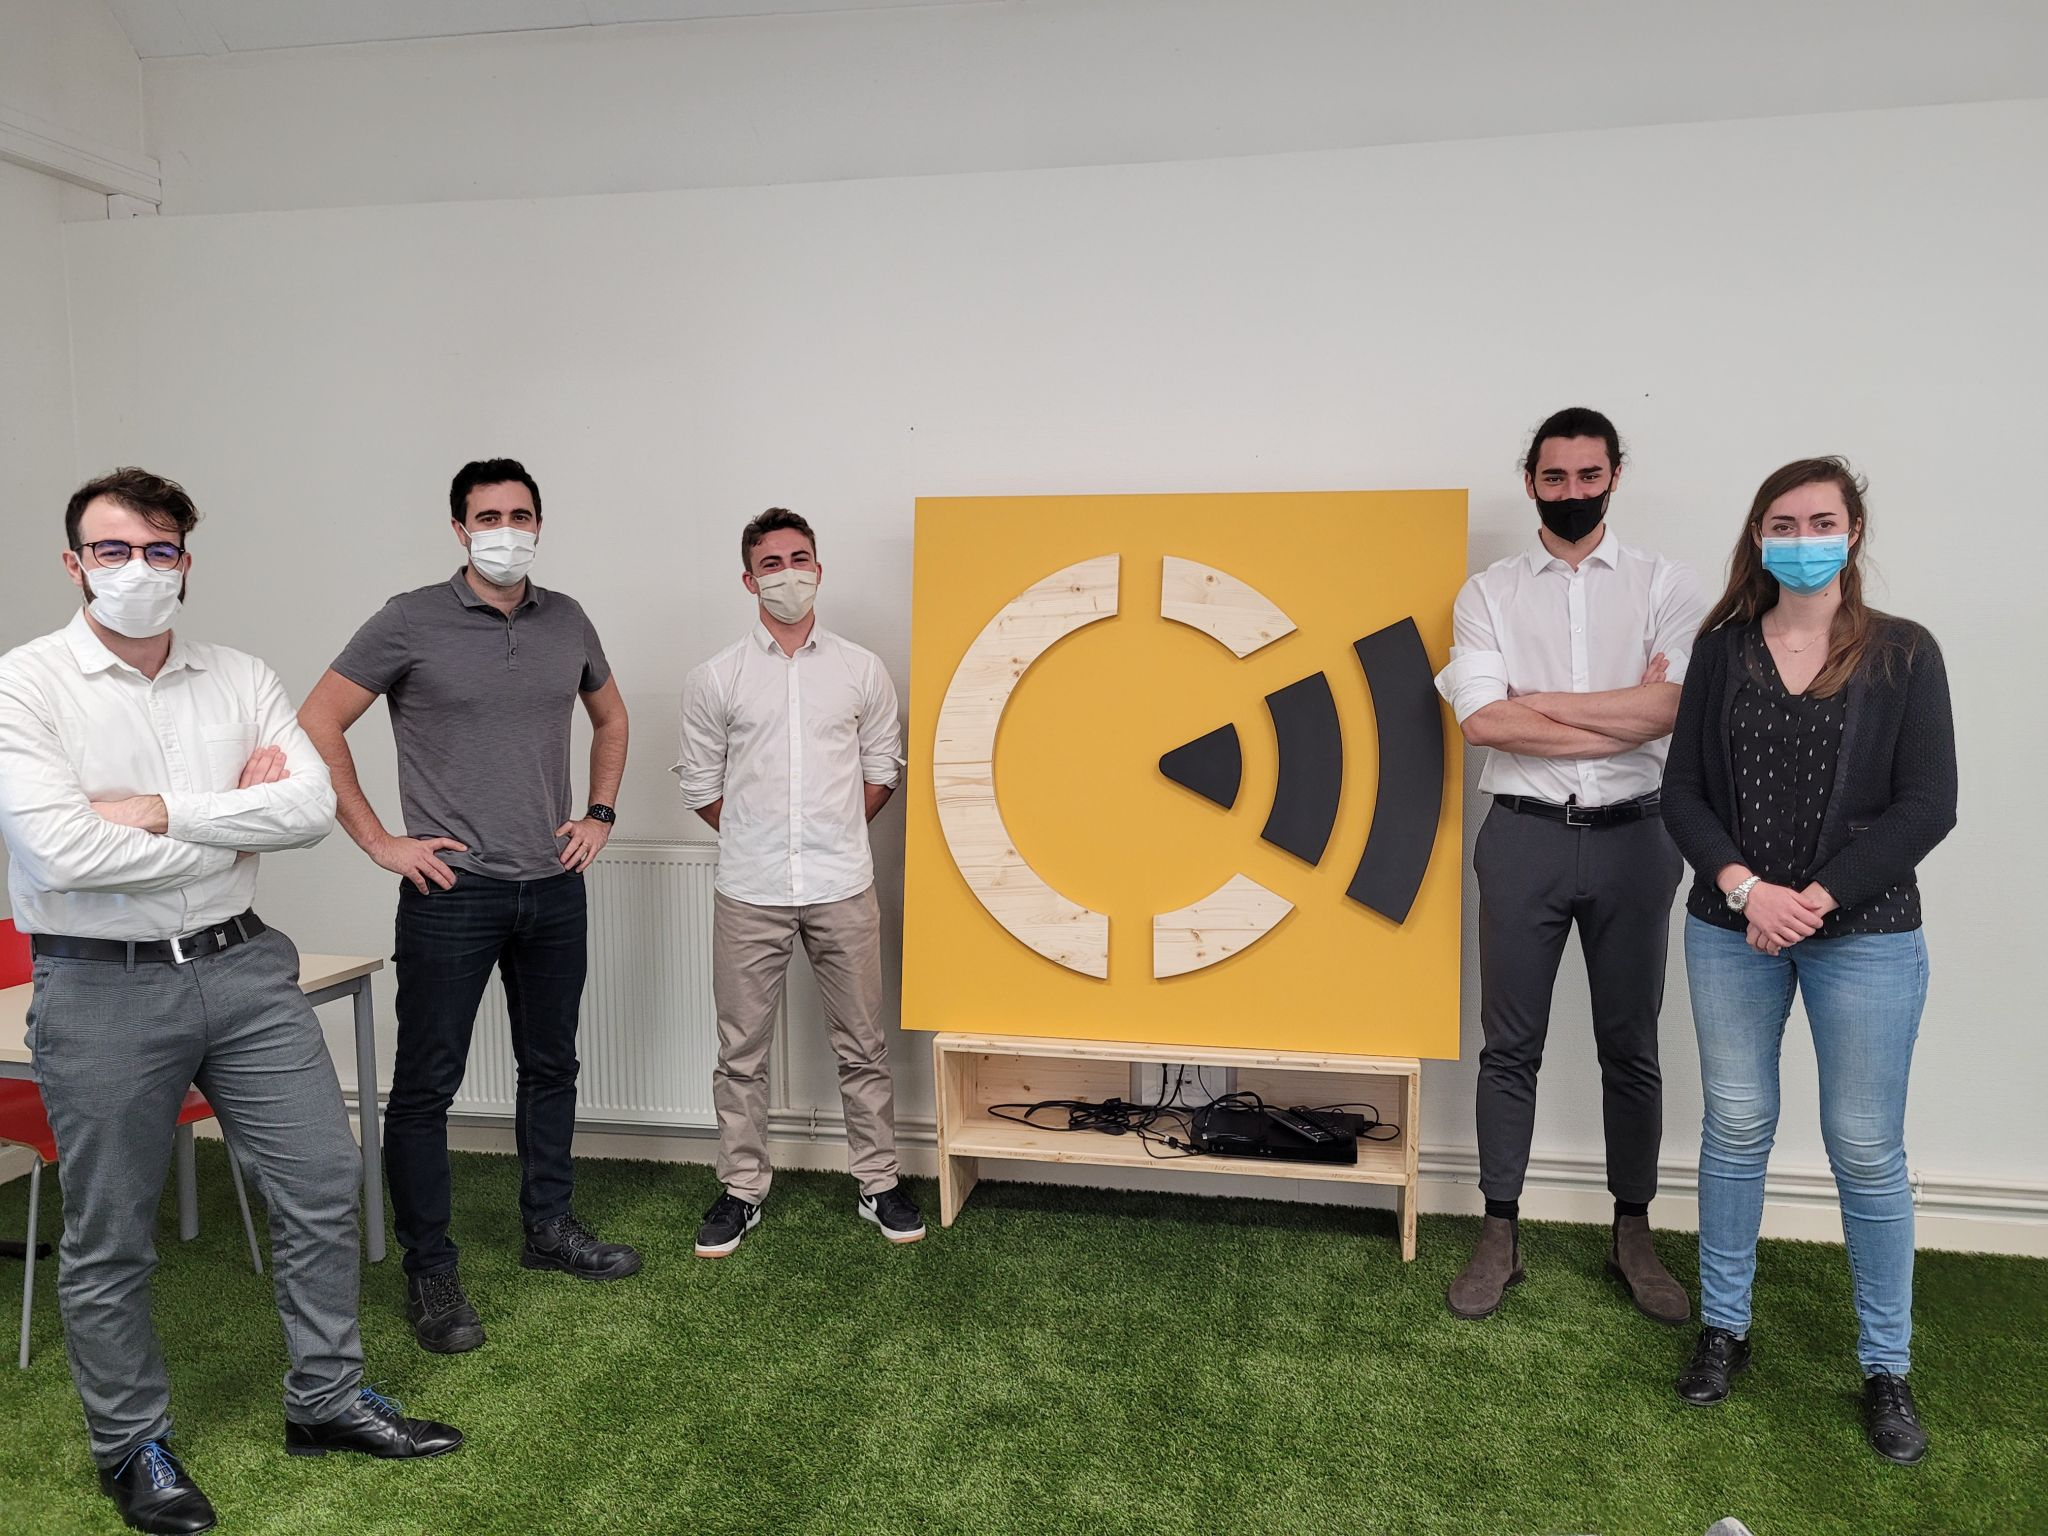
\includegraphics[scale=0.15]{img/team.jpg}
    \caption{\centering Équipe Activ'ESAIP, de gauche à droite: R. \textsc{Girou}, M. \textsc{Lecointre}, C. \textsc{Barbault}, V. \textsc{Carrillo}, J. \textsc{Oudard}}
    \label{fig:Equipe Activ'ESAIP}
\end{figure}

Pour aider les entreprises à s'améliorer, Panorama performance propose plusieurs accompagnements tels que le \textbf{diagnostic DRSO}, des formations en \textbf{Process Communication}, des \textbf{diagnostics de performance} ou encore des \textbf{accompagnements opérationnels}.\\

\clearpage
\subsection{La performance par le séquençage}

Un des outils que Panorama Performance propose aux entreprises suite à ses audits est le \textbf{séquenceur}. Cet outil a pour objectif de donner une vision globale de la charge de travail sur les deux semaines ou le mois qui vient. Panorama Performance adapte sa solution au cas par cas pour s'adapter aux besoins de chacune des entreprises qui s'en voit dotée ; c'est d'ailleurs un des points fort de l'accompagnement de Panorama Performance : la personnalisation de la solution.

\begin{figure}[!h]
    \centering
    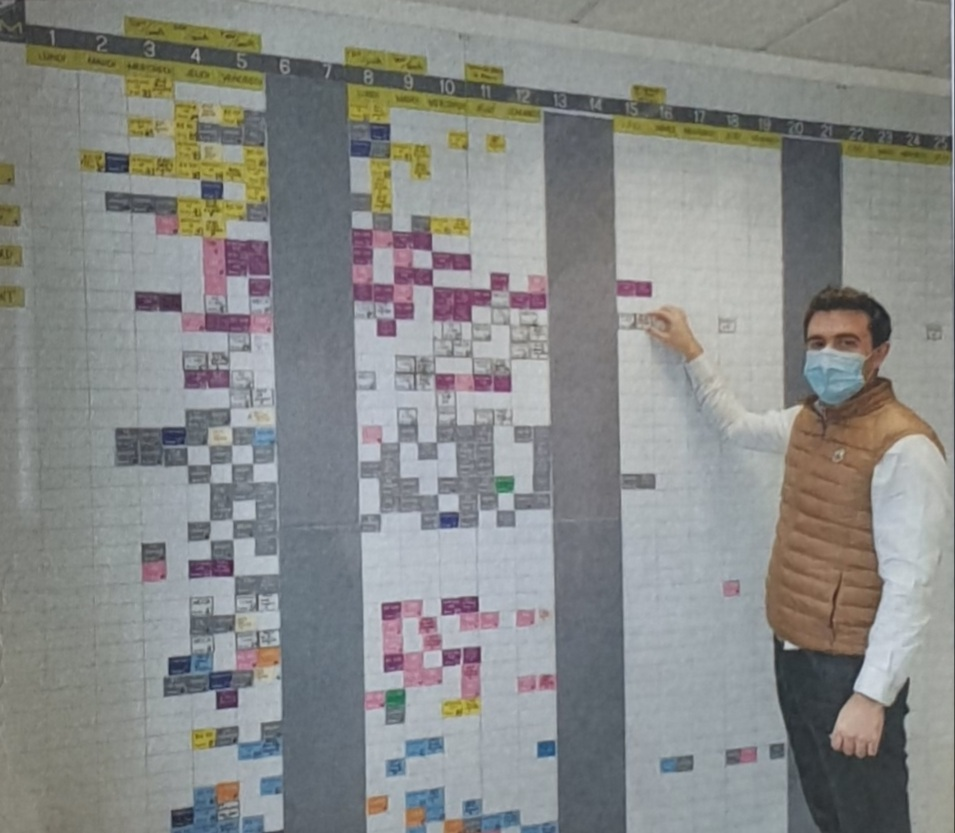
\includegraphics[scale=0.4]{img/sequenceur_2.jpeg}
    \caption{Le séquenceur, un outil d'aide à la performance industrielle}
    \label{fig:Séquenceur}
\end{figure}

De plus, cet outil de gestion de la planification industrielle est interactif : il permet à toute l'équipe de se retrouver afin de pouvoir interagir, communiquer et se mettre d'accord sur les modifications de planning à mettre en place\footnote{Lorsque l'équipe est adaptée à l'outil, seul le manager modifie le séquenceur et l'équipe n'a qu'à le consulter}.\\

\subsubsection*{Principe de fonctionnement}

Après une phase de prototypage de quelques jours, Panorama Performance cible les besoins de ses clients et construit ensuite avec eux un séquenceur. Sur ce séquenceur, on retrouve les commandes client (dans la figure \ref{fig:ProductionItem} elles sont placées dans une colonne à gauche) avec la référence de la pièce.\\

Le responsable vient ensuite placer dans la ligne correspondante toutes les étapes de fabrication nécessaires pour la commande (fraisage, tournage,\dots~cf. figure \ref{fig:productionLigne}). Ces étapes sont initialement les unes à la suite des autres, mais il les déplacera à une date antérieure si la charge de travail de la journée est trop importante ; de cette manière, la production est faite “Juste à temps" !\\

\begin{figure}[!h]
    \centering 
    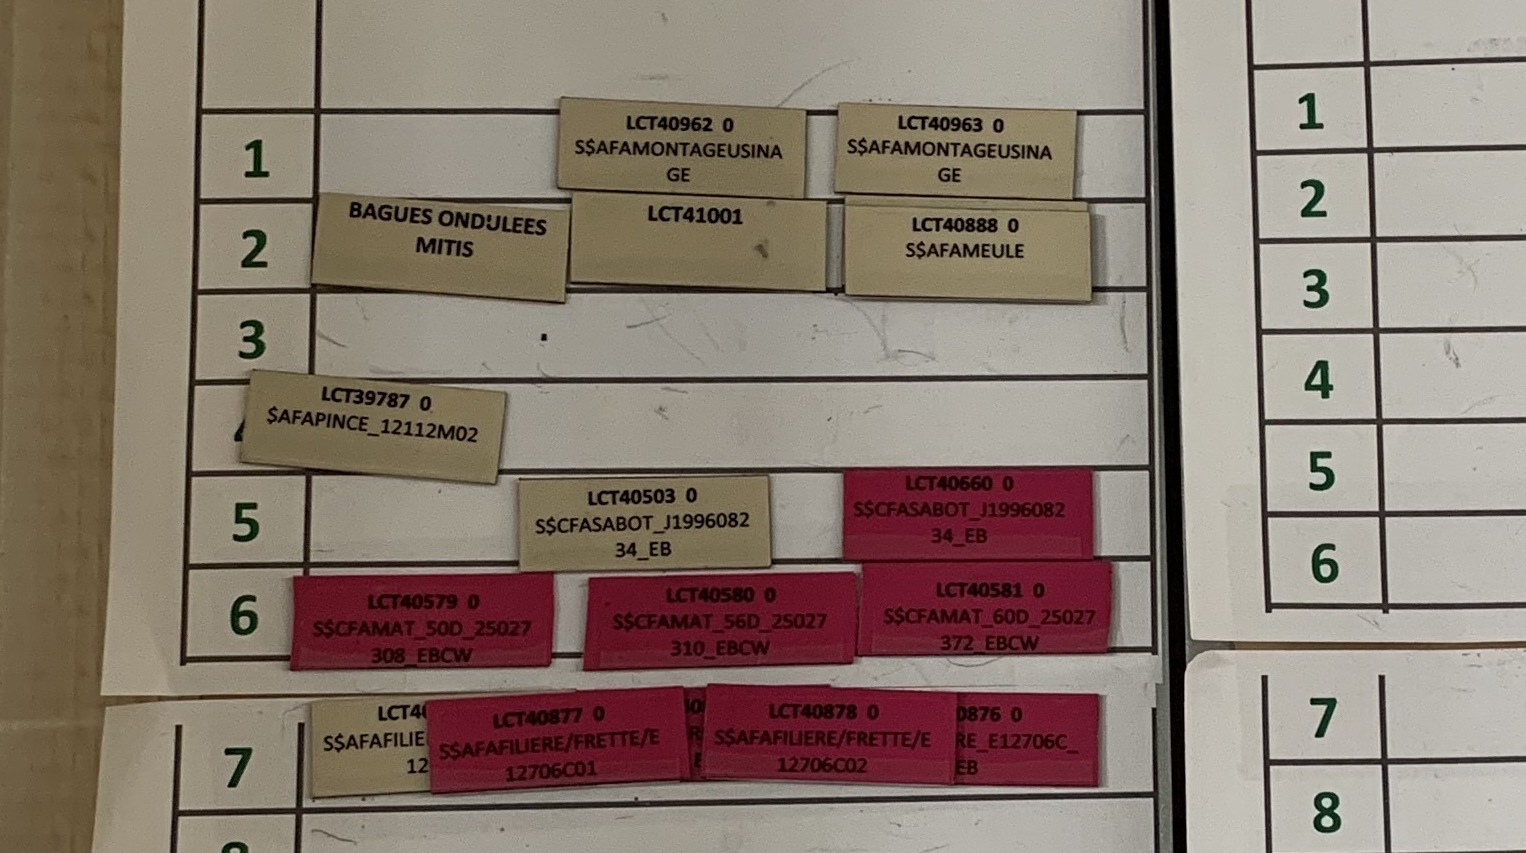
\includegraphics[scale=0.3]{img/productionItem.jpg}
    \caption{Les commandes sont ici placées à gauche}
    \label{fig:ProductionItem}
\end{figure}
\begin{figure}[!h]
    \centering
    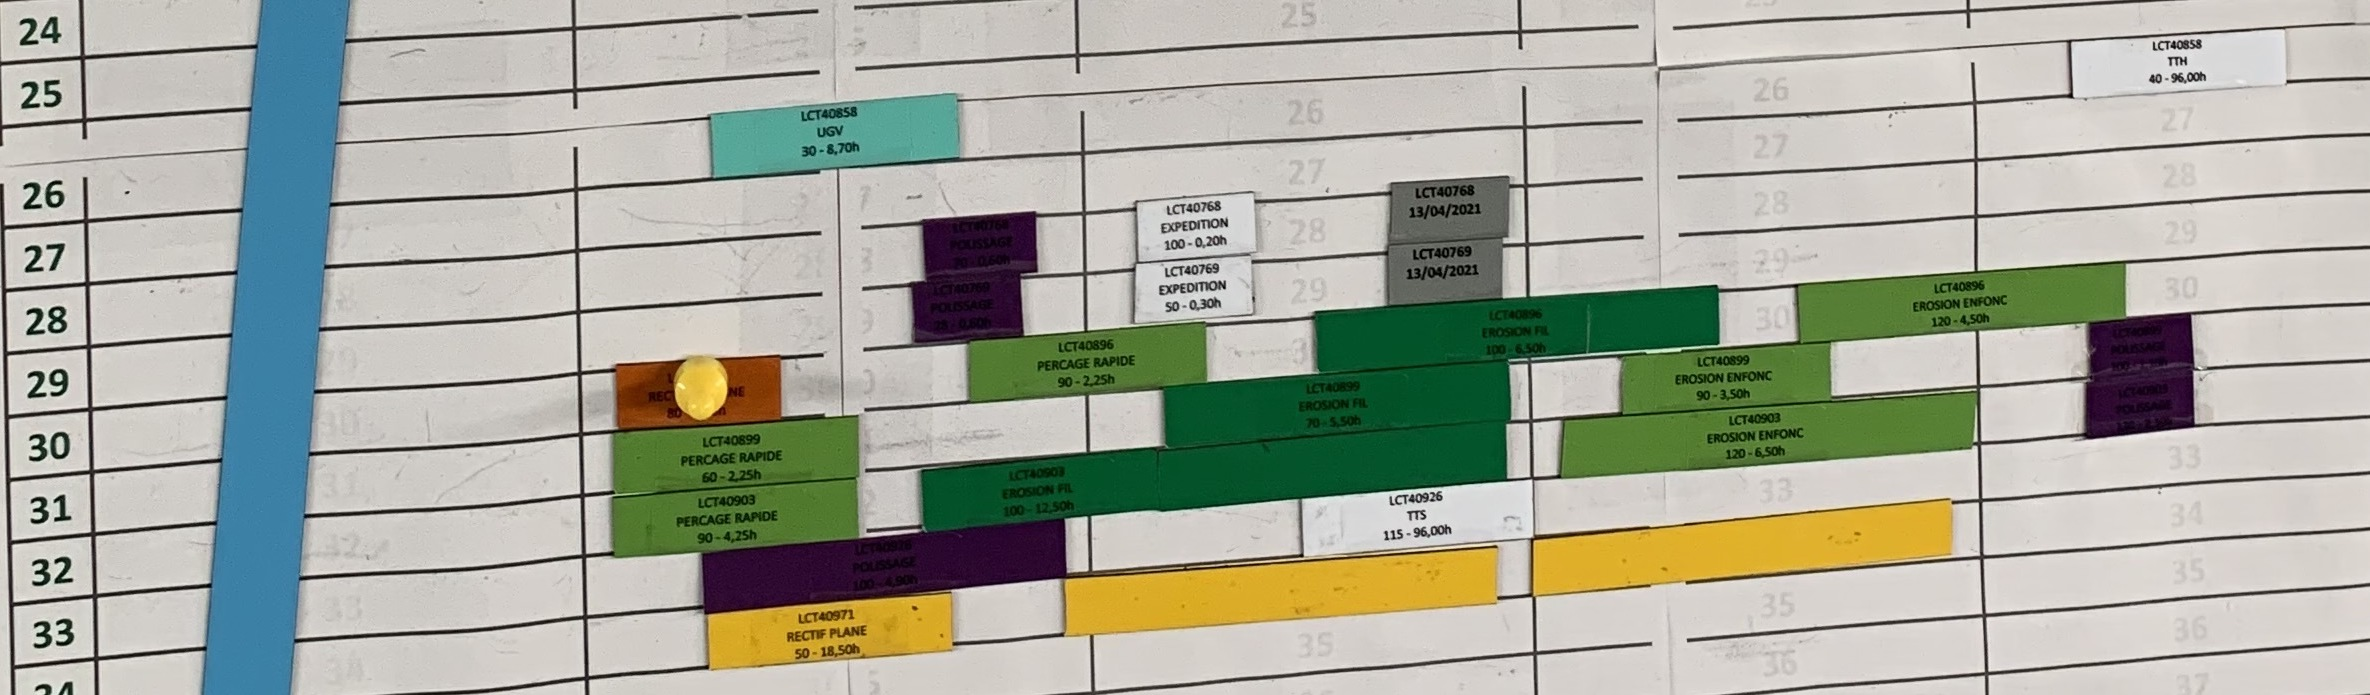
\includegraphics[scale=0.19]{img/ligne_production.jpg}
    \caption{Les lignes de production sont remplies avec les étapes de production}
    \label{fig:productionLigne}
\end{figure}   

Les cartes d'étapes de production ont une couleur associée à leur tâche, et une longueur variable en fonction de la charge horaire associée. Le nom de la compétence, la quantité de pièces à effectuer, la durée,\dots toutes ces informations figurent sur la carte, elles sont donc longues à réaliser à la main, et certains clients se dotent même d'imprimante à étiquette pour accélérer cette étape.
\hfill \\


\begin{figure}[!h]
    \centering
    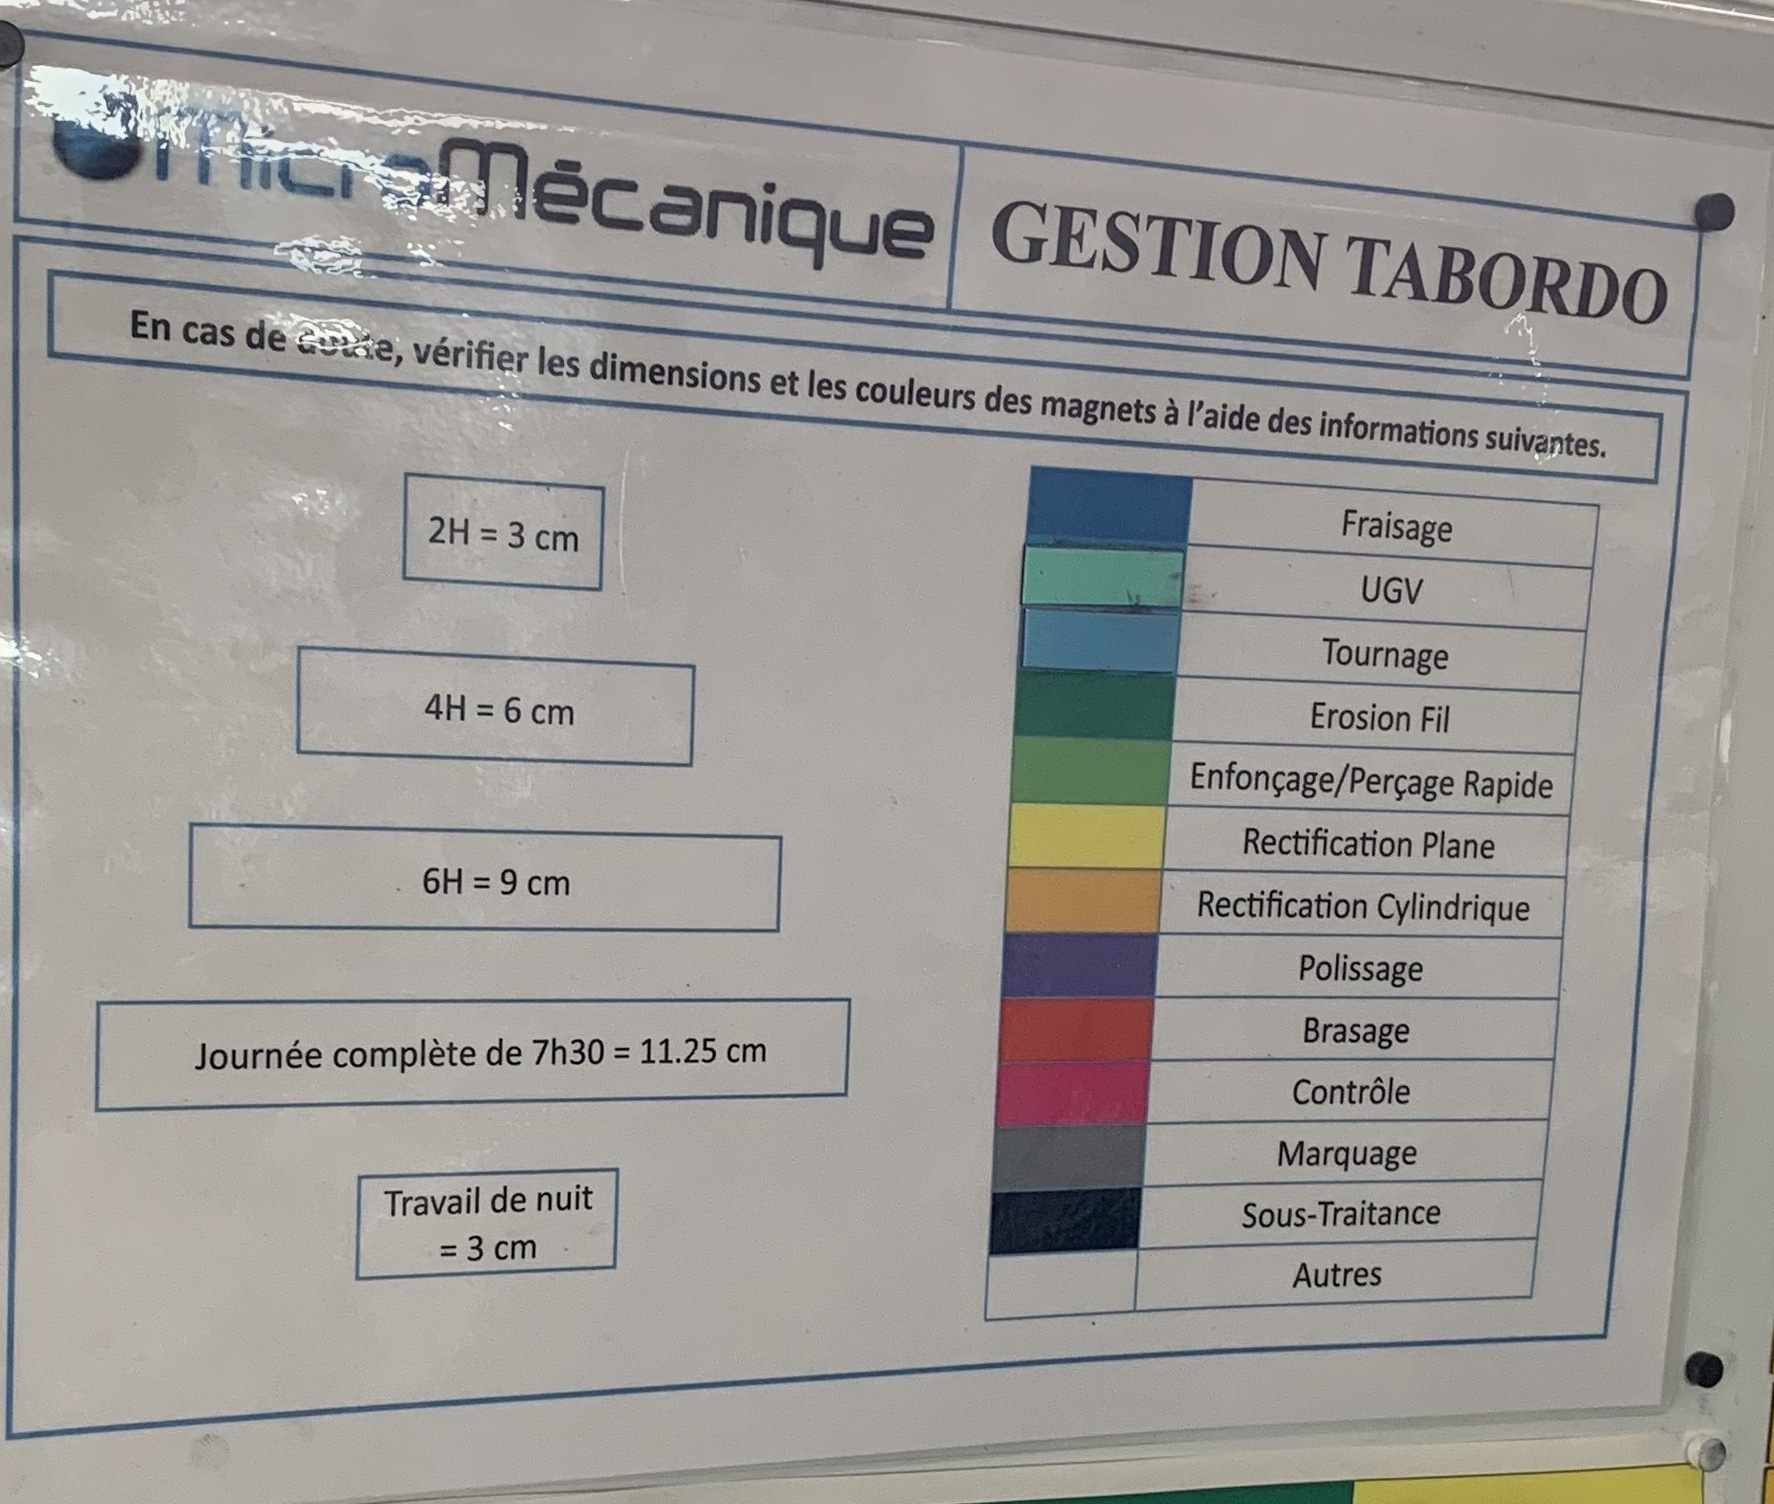
\includegraphics[scale=0.2]{img/productionStep.jpg}
    \caption{Les cartes d'étape de production suivent un design codifié (couleur, taille, contenu,\dots)}
    \label{fig:productionStep}
\end{figure}

Enfin, le manager peut placer des vignette (ici des épingles de couleur, cf. figures \ref{fig:productionLigne} et \ref{fig:employee}) pour signaler à chaque employé quelle sera sa mission du jour.

\begin{figure}[!h]
    \centering
    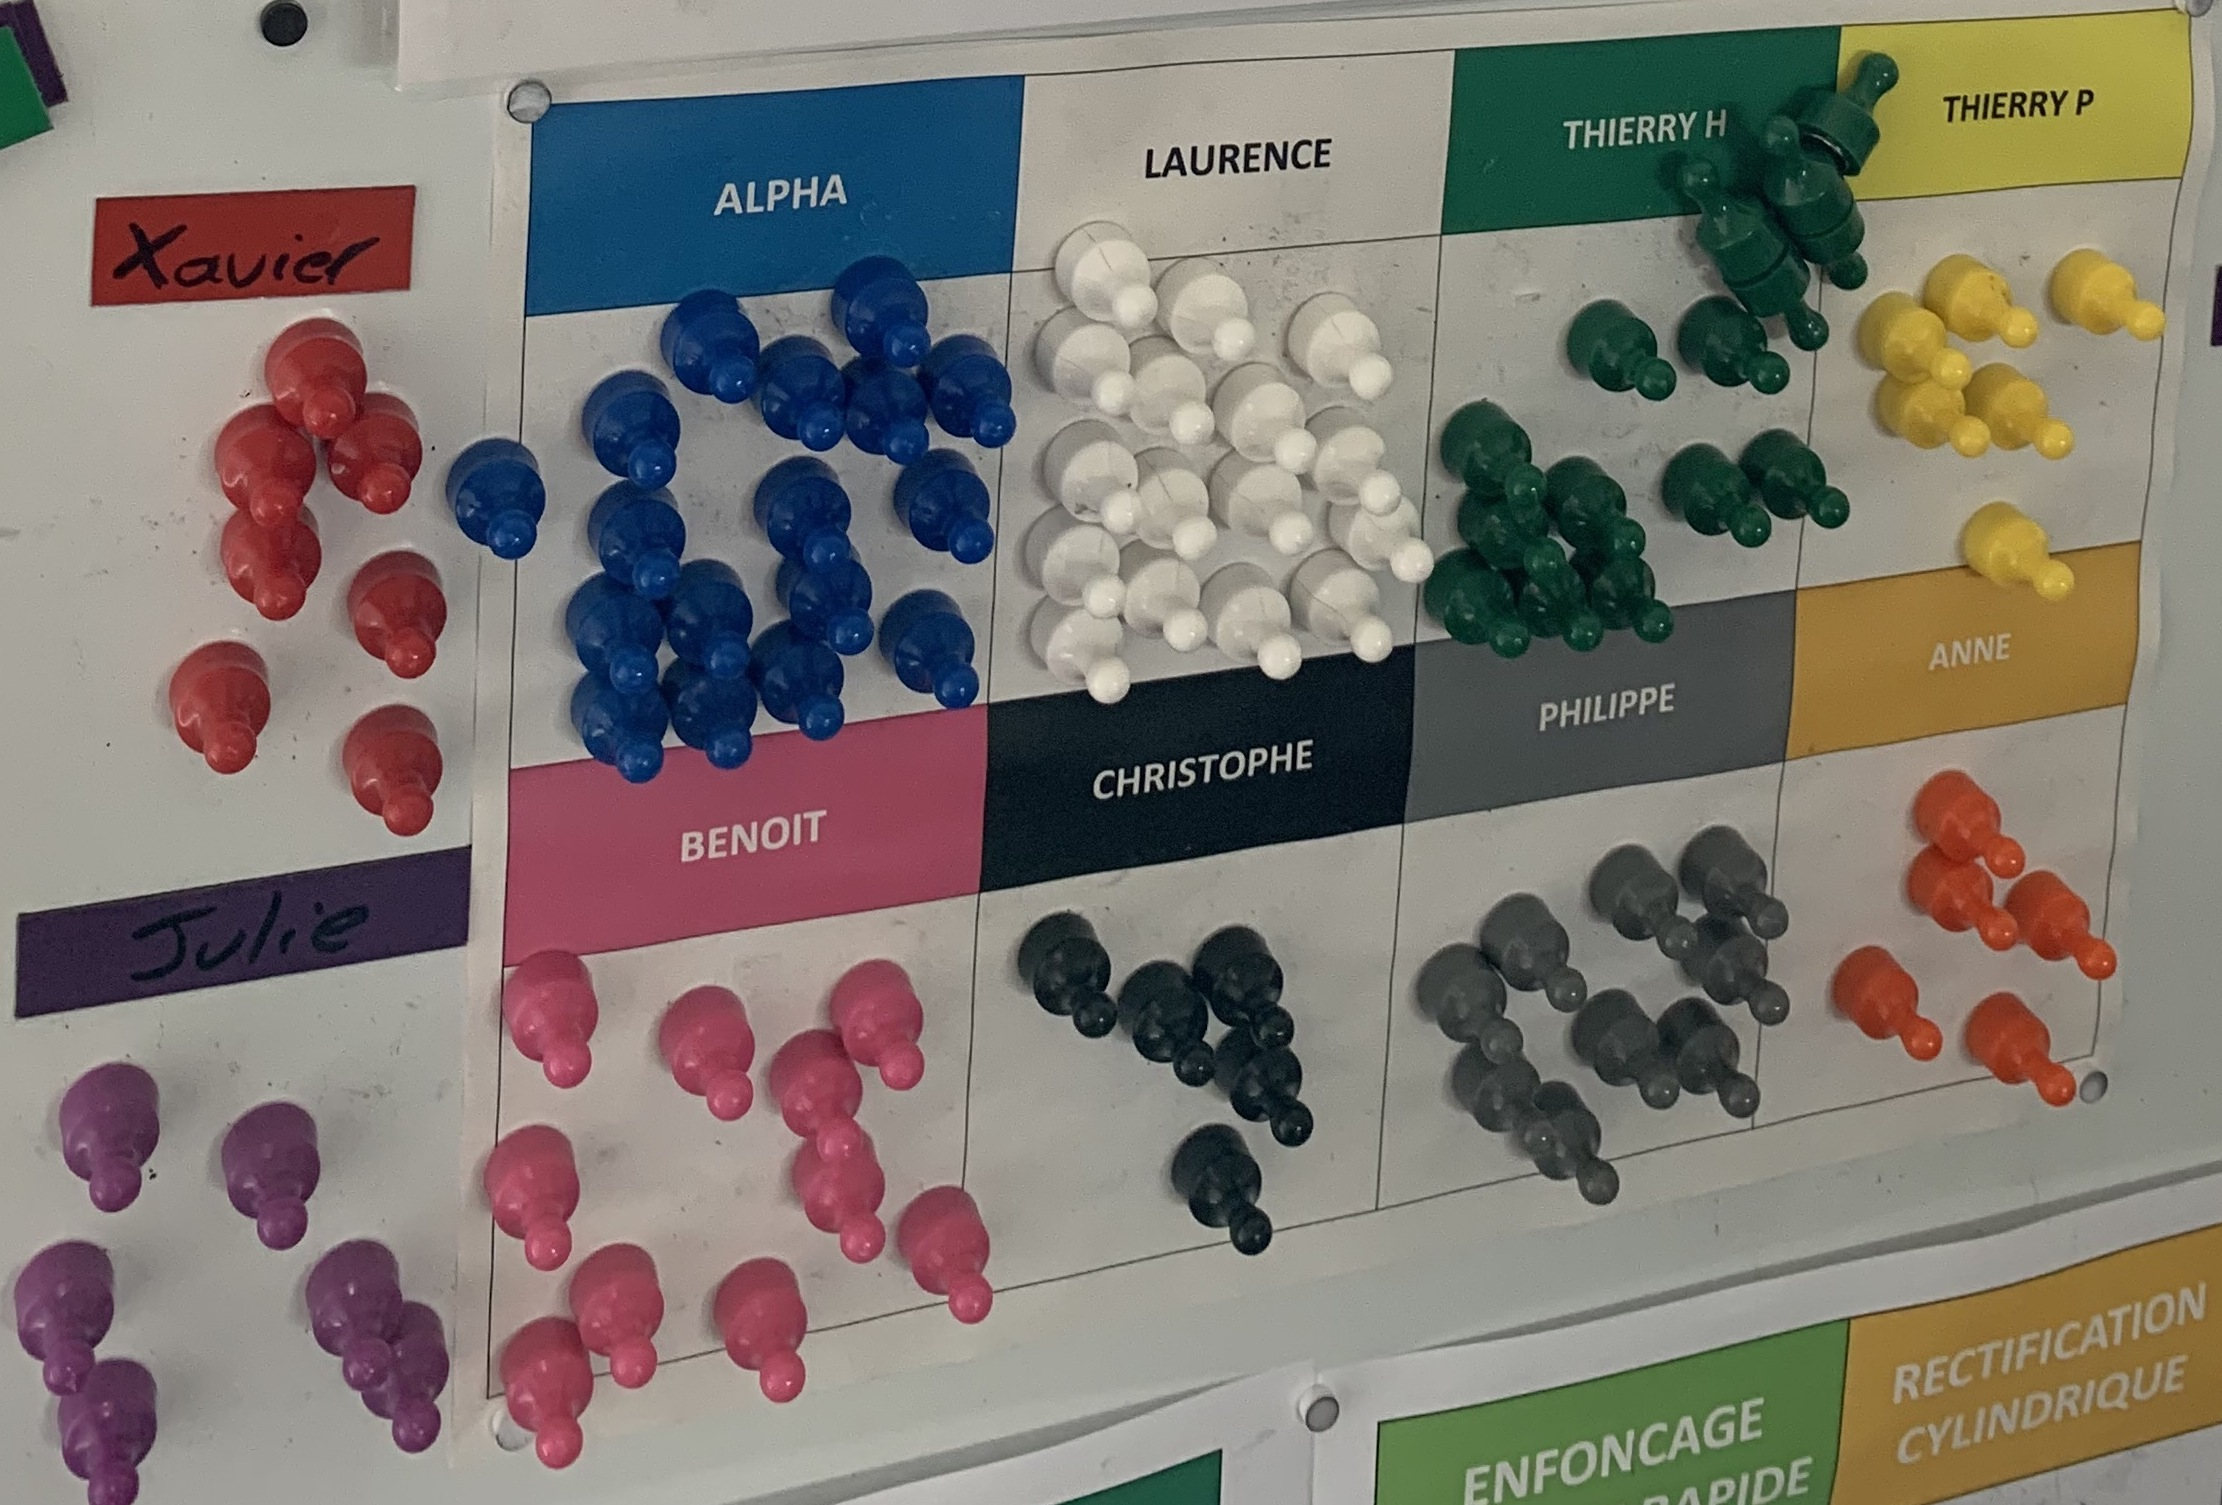
\includegraphics[scale=0.15]{img/employee.jpg}
    \caption{Chaque employé a sa couleur d'épingle pour identifier ses missions}
    \label{fig:employee}
\end{figure}

\hfill \\
Cet outil a permis à Panorama de se démarquer de ses concurrents (comme "maboutiqueenlean"\cite{MaBoutiqueEnLean} par exemple) qui eux, ne font pas réellement de l'accompagnement global des TPE personnalisé.


\clearpage
\subsubsection*{Problématique}
Mais la version actuelle du séquenceur soulève plusieurs problèmes : 
\begin{itemize}
    \item Il est encombrant
    \item L'aspect “papier/crayon" repousse les entreprises
    \item Son utilisation est gourmande en temps
\end{itemize}

C'est pourquoi Panorama Performance s'est posé la question d'un possible passage à une solution informatique reprenant les éléments clés de cet outil. L'application qu'ils souhaiteraient mettre place devra permettre de laisser les collaborateurs réfléchir aux modifications qui les arrangent et interagir entre eux pour trouver leur propre façon de gérer la production de manière optimisée. Panorama Performance a fortement insisté sur le fait qu'il nous fallait \textbf{digitaliser et conserver les fonctionnalités actuelles sans automatiser} !\\

La dernière proposition de valeur de ce projet serait de pouvoir mettre en place, un backup des données des utilisateurs (délais de livraison, disponibilité des machines, productivité, \dots) Cela permettra, grâce à ces informations, à la demande des clients, de créer des indicateurs qui permettront, d'améliorer encore la performance.


\setcounter{section}{1}
\include{tex/mission_methodologie}
\section{Mission}
\subsection{Choix des technologies}

\subsubsection*{Flutter}
\addcontentsline{toc}{subsubsection}{Flutter}


Pour réaliser la POC, nous avons décidé d'utiliser le framework Flutter de Google\cite{Flutter}. Ce framework permet le développement d'applications cross plate-formes natives\footnote{sur Android, IOS, Web, Linux, Windows et Mac}.

\begin{figure}[h!]
    \centering
    
\includegraphics[scale=0.5]{img/Flutter.jpg}
    \caption{Flutter, un framework Google cross-plateforme}
    \label{fig:Flutter logo}
\end{figure}

Bien que décrié par certain comme une simple tendance ou un framework non-viable sur le long terme, Flutter s'est pourtant hissé à la première place en terme de framework cross-plateforme avec 45\% de votes\footnote{D'après une étude menée par SlashData\cite{Flutter2.2}}. Des entreprises telle que \textbf{BMW}, \textbf{Tencent} (avec son application WeChat utilisée par 1.2 Milliards d'utilisateurs), ou encore \textbf{Toyota} \footnote{Flutter sera au cœur du système d'infotaienment de la prochaine génération de véhicules.} l'utilisent ; même des projets open-source de grande ampleur comme \textbf{Ubuntu} s'y sont mis \footnote{la totalité de l'installer a été redesigné en Flutter\cite{UbuntuFlutter}}.\\

\begin{figure}[!h]
    \centering
    
\includegraphics[scale=0.33]{img/Apps_flutter.png}
    \caption{Quelques applications codées à l'aide de Flutter}
    \label{fig:my_label}
\end{figure}

Flutter est très orienté design responsive, les interfaces créées avec s'adaptent donc à toutes les tailles d'écran. De par sa compatibilité avec les smartphones, Flutter propose de nombreux packages utilisables par tactile, il s'imposait comme une technologie de choix pour nous.\\
De plus, notre team de développeurs était déjà formé à cette technologie et avait déjà réalisé plusieurs projets avec ce framework, que ce soit en cours ou en entreprise.\\

Depuis sa version 2.0 sortie début mars 2021, Flutter supporte le développement Web depuis sa branche \texttt{stable}. Il est même proposé aux utilisateurs de télécharger la web app sur leur appareil lorsqu'ils se rendent sur le site.\\
Nous avons donc concentré nos efforts sur cette plateforme, mais une application mobile peut être une piste pour le projet final.

\subsubsection*{Firebase}
\addcontentsline{toc}{subsubsection}{Firebase}

Pour ce qui est du stockage des données, nous avons porté notre choix sur \textbf{Firebase}, la solution de base de données \textbf{NoSQL}\footnote{“Non-SQL" ; les bases de données NoSQL sont, à l'inverse des bases de données SQL, non-structurées, d'où leur nom.}\cite{NoSQL} de Google\cite{Firebase}. Comme Flutter et Firebase sont deux technologies de Google, il est donc très facile de les coupler. Cette plateforme est gratuite en dessous des 10 k écriture/lectures par mois, ce qui est très largement suffisant pour une POC.\\

\begin{figure}[h!]
    \centering

\includegraphics[scale=0.15]{img/firebase.png}
    \caption{Firebase, la solution de base de données NoSQL Google}
    \label{fig:Firebase Logo}
\end{figure}

D'après notre expérience en développement, la forte disponibilité de cette solution en fait l'outil parfait pour une application professionnelle. En effet, comme la totalité de la base de données est hébergée par Google, Panorama Performance n'aura pas à se soucier de la sécurité des données (redondance, sauvegarde, cryptage), ni de la gestion d'un serveur (maintenance, scalabilité horizontale et verticale, \dots).\\

\begin{figure}[!h]
    \centering
    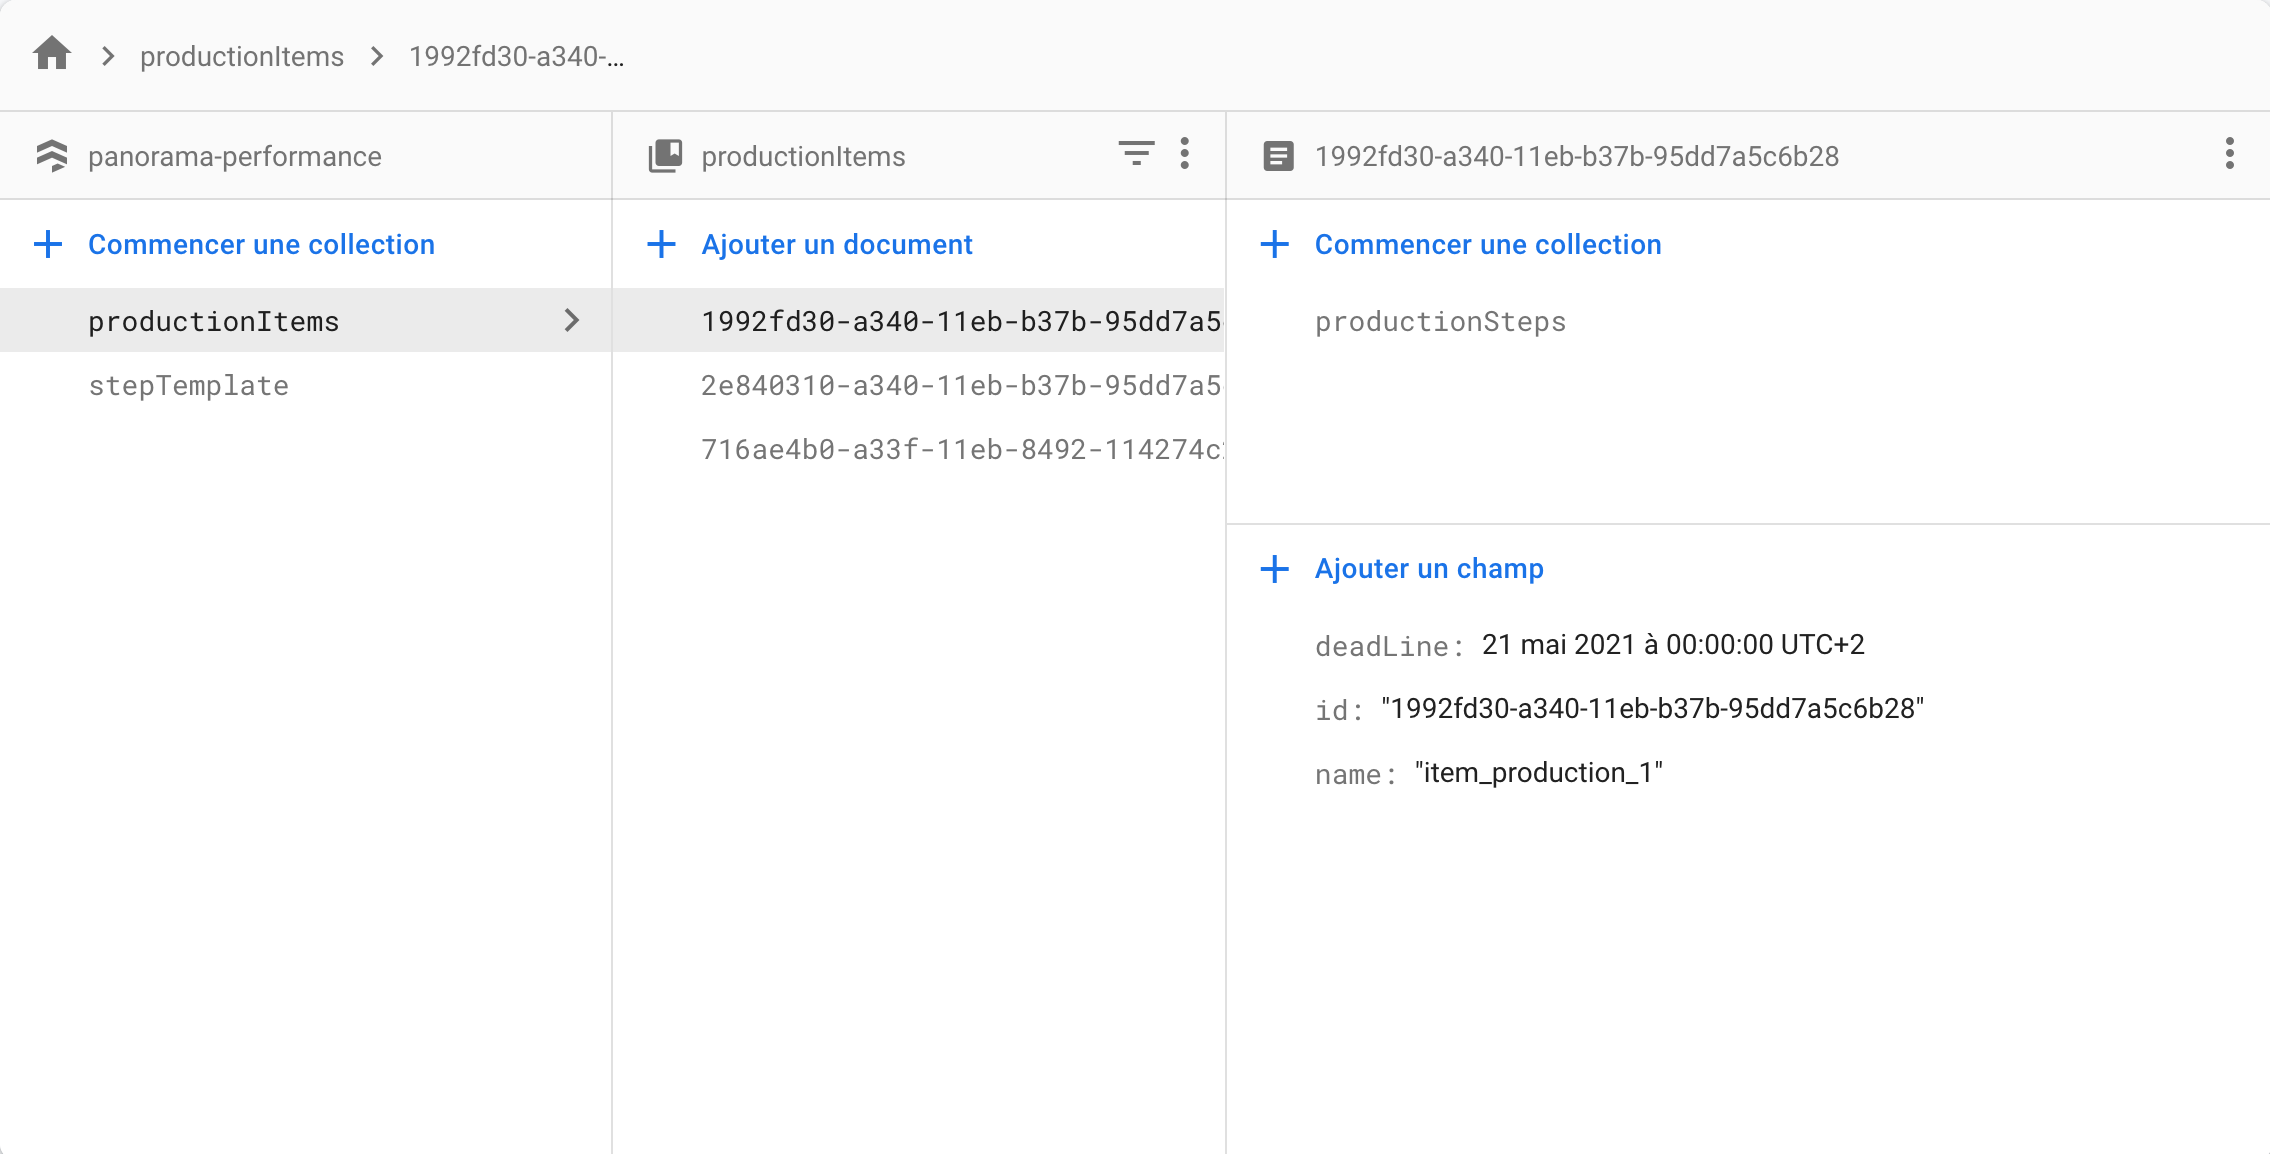
\includegraphics[scale=0.2]{img/screen_firebase.png}
    \caption{Capture d'écran de la base de données NoSQL au 20 mai 2021}
    \label{fig:CaptureFirebase}
\end{figure}

\begin{figure}[!h]
    \centering
    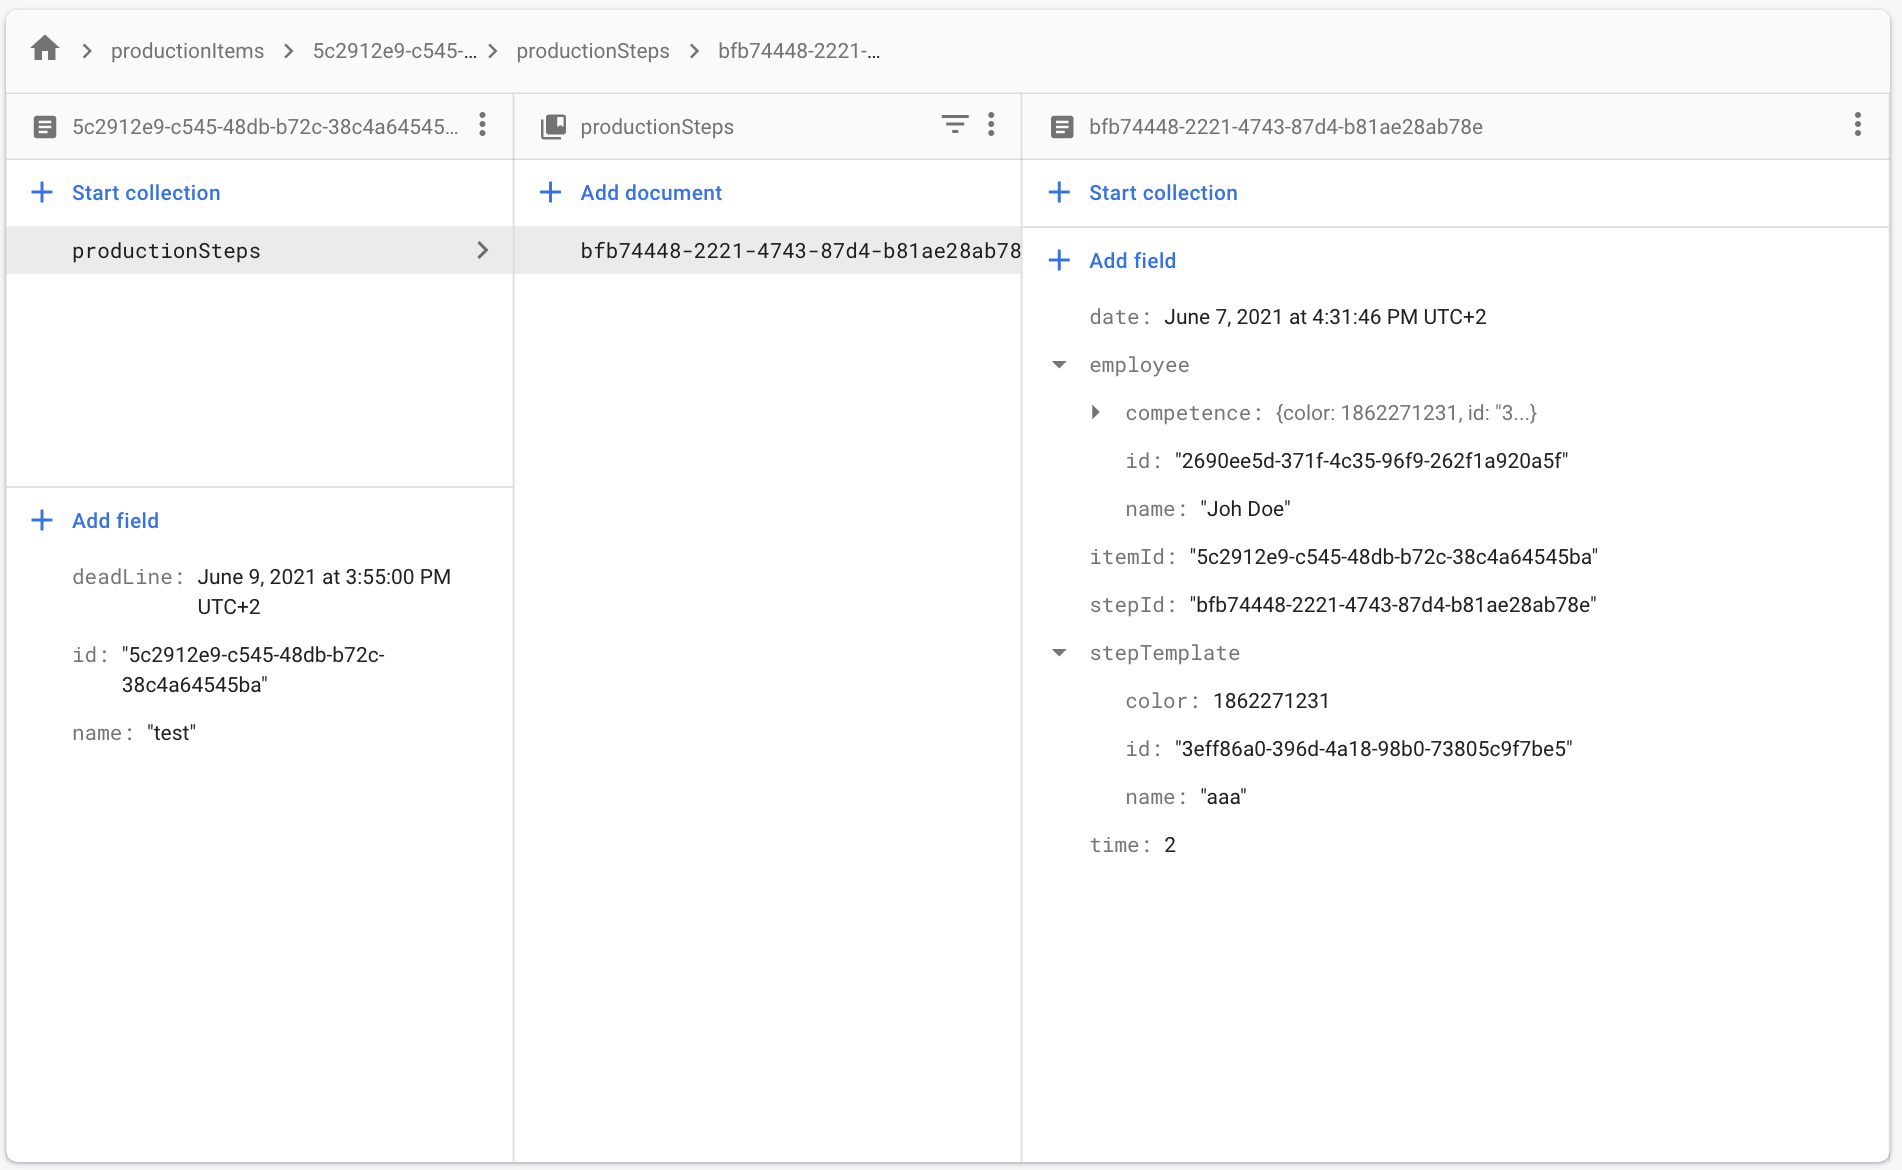
\includegraphics[scale=0.5]{img/screen_firebase2.png}
    \caption{Capture d'écran de la base de données NoSQL au 4 juin 2021}
    \label{fig:CaptureFirebase}
\end{figure}

Firebase étant une base de données NoSQL avec un stockage sous format de document\footnote{Documents JSON pour être plus précis.}, il est ainsi très facile d'accéder à n'importe quelle propriété d'un document particulier, et cela même si le document est lui-même stocké au sein d'une collection.(cf. Fig. \ref{fig:CaptureFirebase})

\clearpage
Nous avons opté pour le design de classe suivant : 

\begin{figure}[!h]
    \centering
    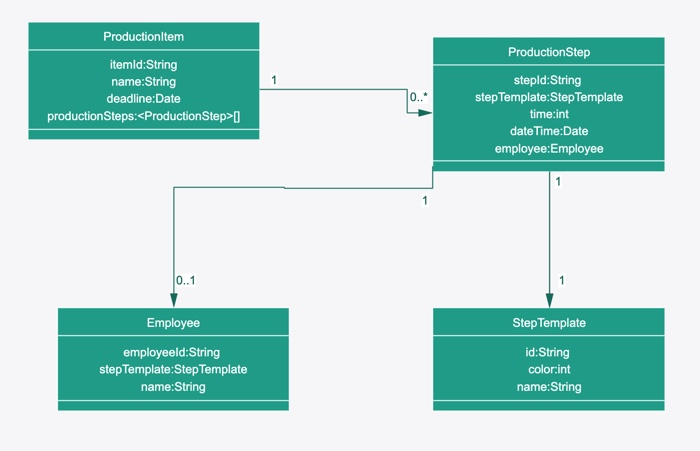
\includegraphics[scale=0.6]{img/class_diag.jpeg}
    \caption{Design de la base de données}
    \label{fig:diagClass}
\end{figure}


\subsection{Gestion de projet}

\subsubsection*{Méthode agile}
\addcontentsline{toc}{subsubsection}{Méthode Agile}

Lors de ce projet, nous avons, d'un commun accord entre nous 3 et Panorama Performance, décidé de mettre en place un système de management agile.\cite{Atlassian} En effet, le format de sprint\cite{Sprint} de 1 semaine s'adaptait parfaitement au concept de l'activ'Esaip.\\ 
\begin{figure}[h!]
    \centering
    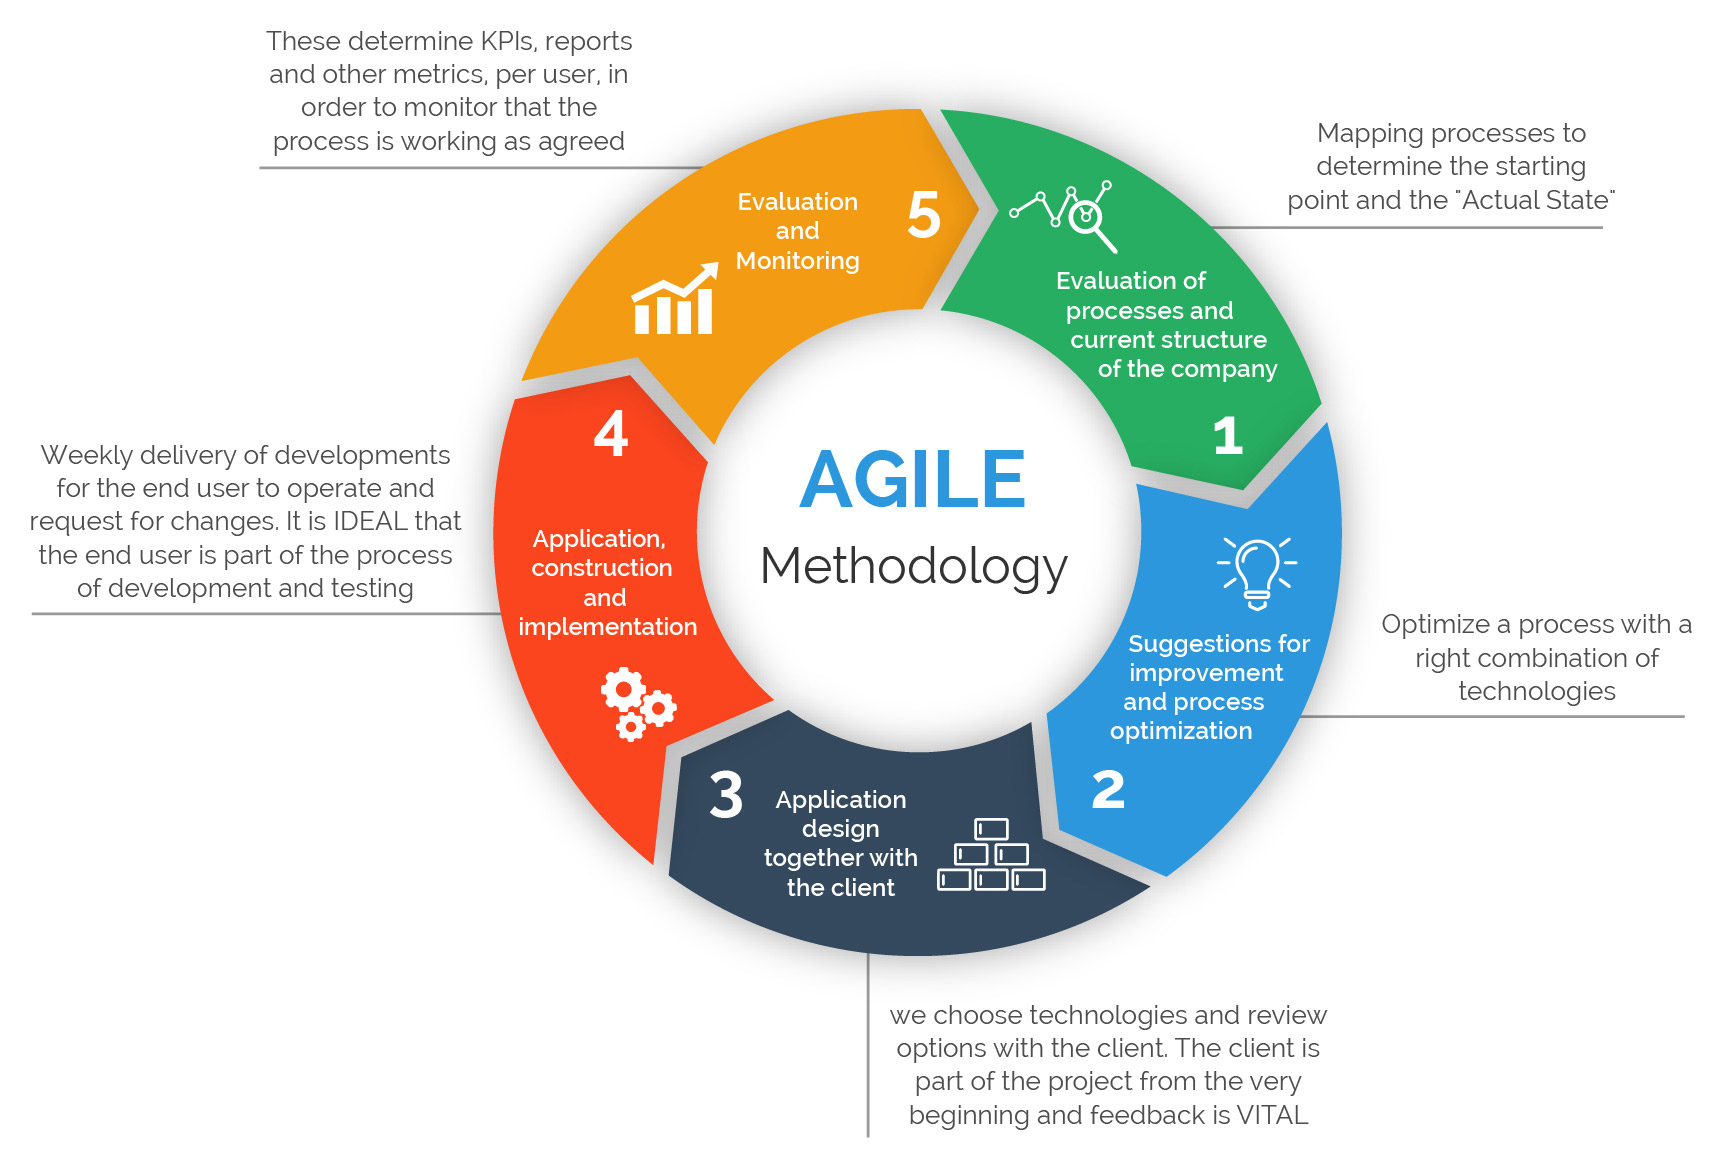
\includegraphics[scale=0.25]{img/agile.jpg}
    \caption{La méthodologie agile place le client au centre du projet.}
    \label{fig:Agile}
\end{figure}

Le management agile repose sur un système itératif ou les remarques du client sont prise en charge après chaque sprint pour apporter des modifications à la solution en cours de développement. 

\subsubsection*{Le client}
\addcontentsline{toc}{subsubsection}{Le client}
Dans le cadre de ce projet, nous avons considéré Panorama Performance comme le \textbf{client}, à chaque réunion de fin de sprint, nous faisions un bilan avec Mme. Oudard et/ou M. Lecointre pour rendre compte de l'avancement et prendre en compte leurs remarques pour le sprint suivant.\\

\subsubsection*{Le product owner}
\addcontentsline{toc}{subsubsection}{Le Product Owner}
Nous avons également désigné M.Oudard comme \textbf{product owner}\cite{ProductOwner} ; en tant que représentante de l'entreprise au sein de l'équipe, elle s'est chargée d'interpréter les besoins de l'entreprise pour en faire des outils fonctionnels.

M. Barbault s'est occupé de remplir le \textbf{backlog}\footnote{Planification hiérarchique des tâches} avec les \textbf{user stories}\footnote{Description simple d'un besoin du client} qu'elle nous communiquait.

\subsubsection*{Le scrum master}
\addcontentsline{toc}{subsubsection}{Le Scrum Master}


Dans la gestion de projet agile, le \textbf{scrum master}\cite{ScrumMaster} est un peu le coach de l'équipe ; il guide le projet dans la bonne direction sans pour autant être considéré comme un chef ou responsable. C'est également la représentation du management agile au sein de l'équipe : il aide à appliquer la méthodologie agile en donnant des conseils aux membres de l'équipe.

\begin{figure}[!h]
    \centering
    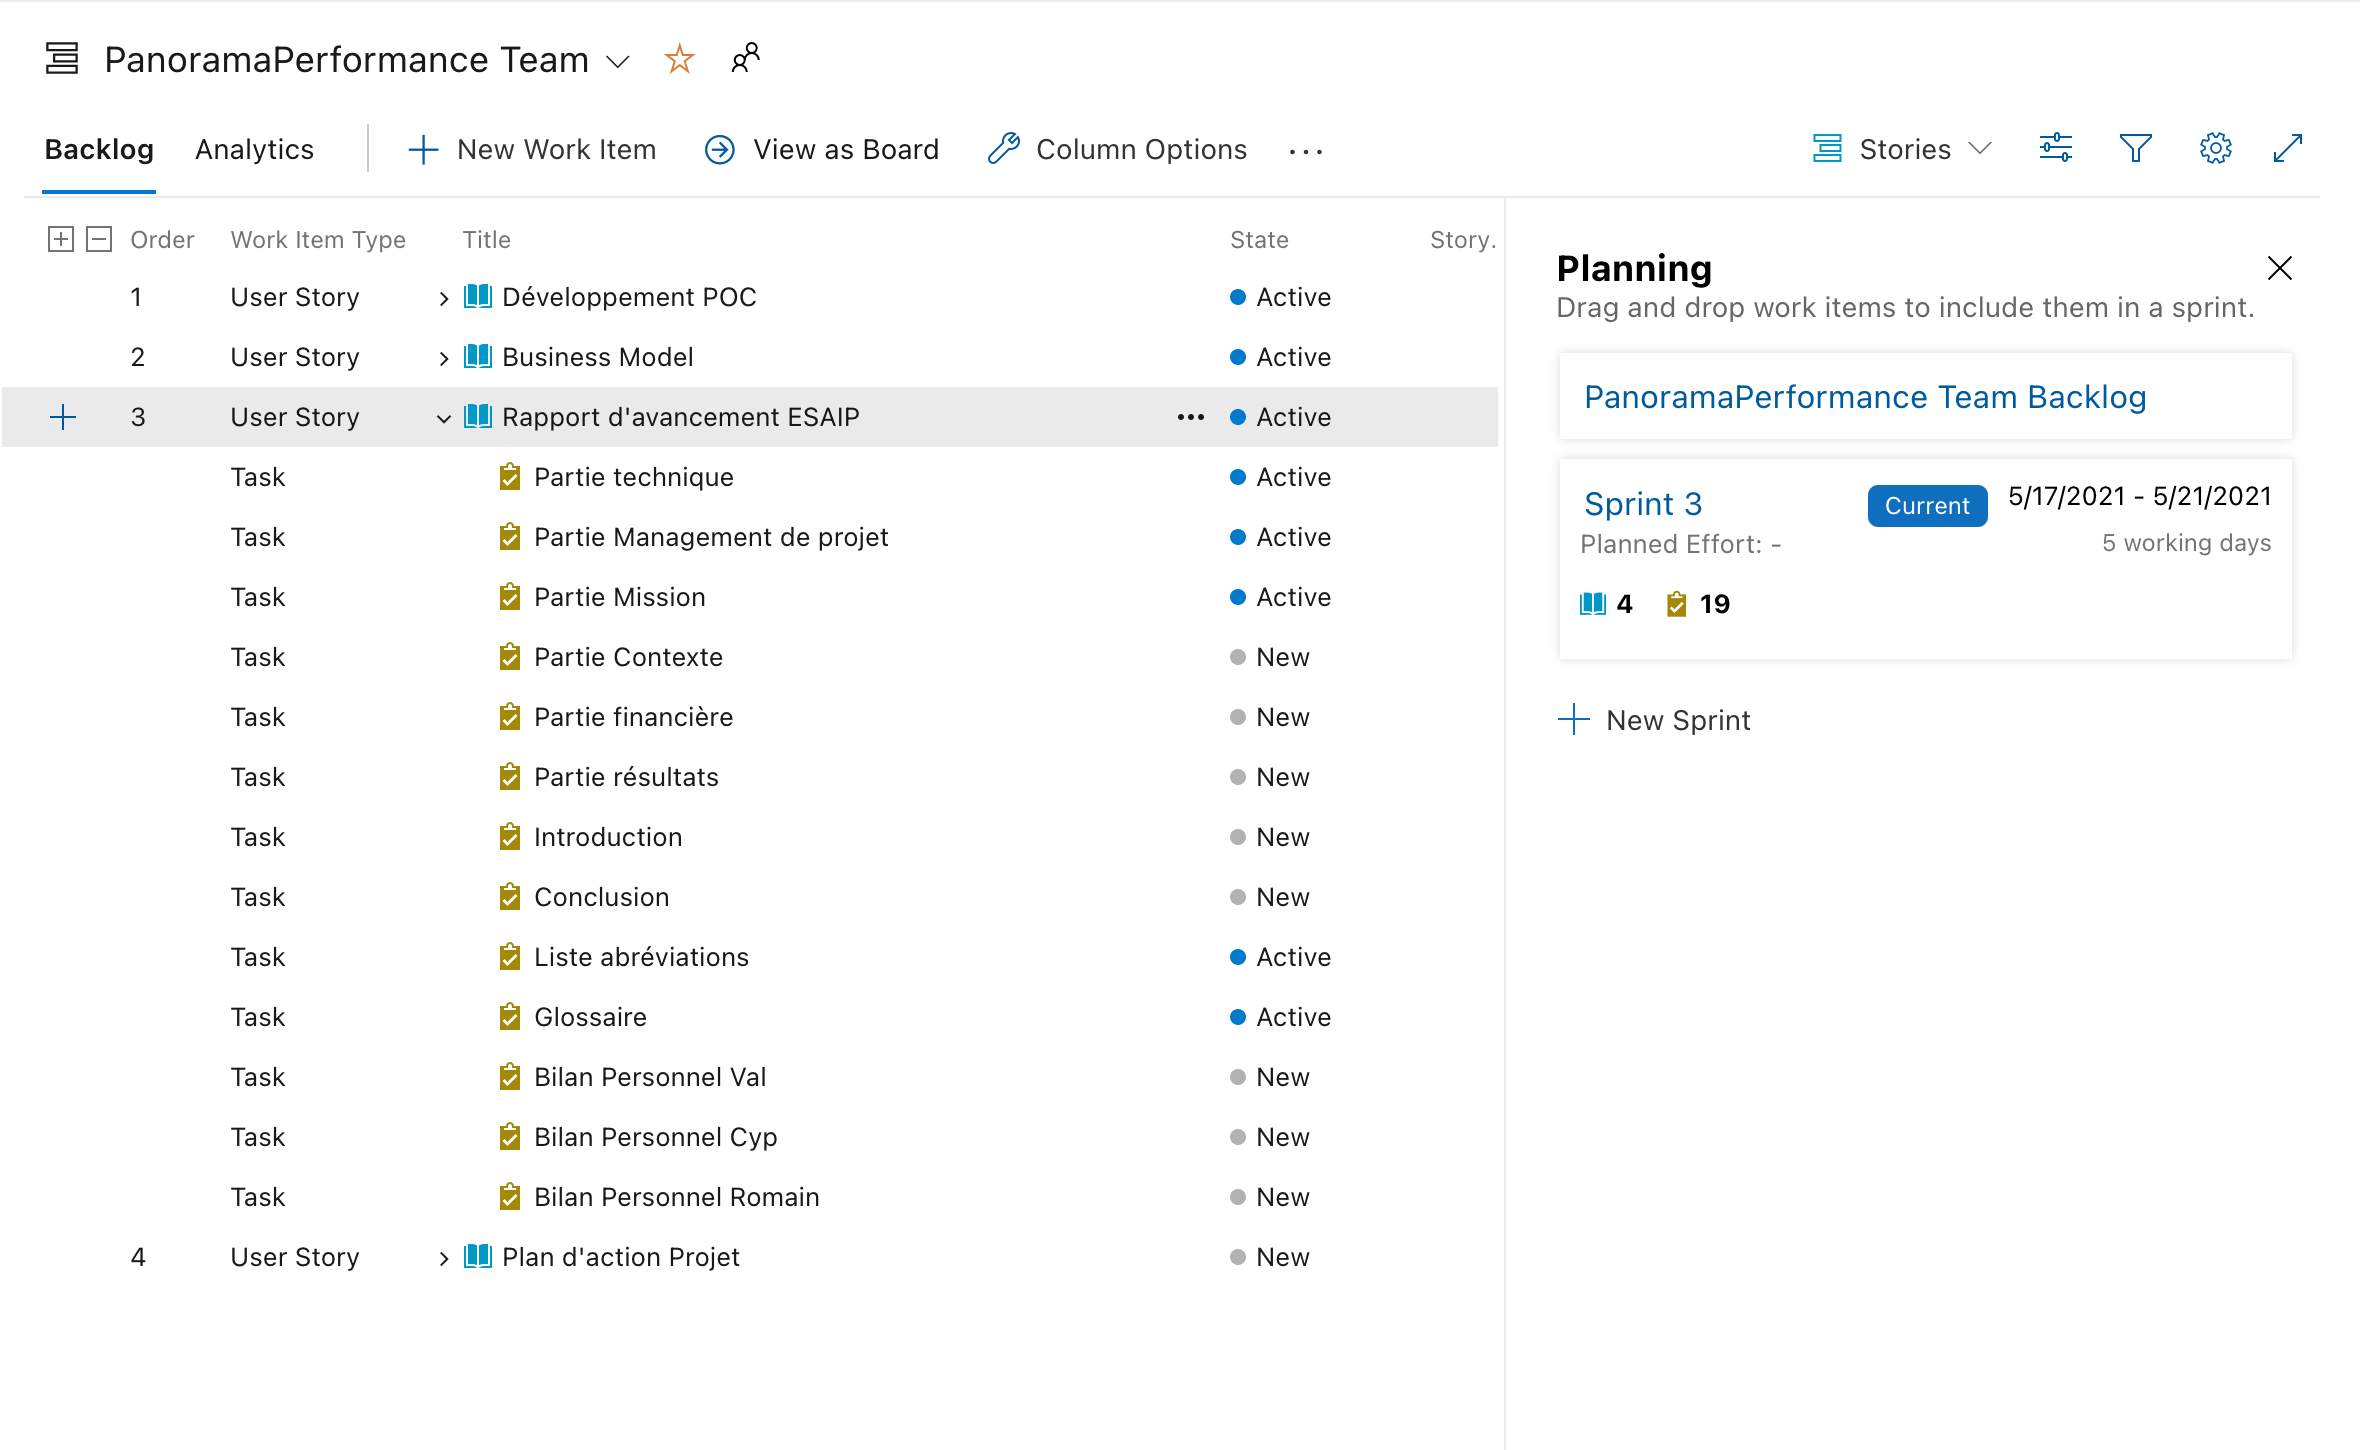
\includegraphics[scale=0.18]{img/backlog.png}
    \caption{Le backlog de notre projet lors du $3^{e}$ sprint}
    \label{fig:my_label}
\end{figure}

\subsubsection*{Déroulement d'un sprint}
\addcontentsline{toc}{subsubsection}{Déroulement d'un sprint}

Chacun des 5 sprints réalisés chez Panorama Performance s'est déroulé selon le même schéma : 
\begin{enumerate}
    \item Réunion de début de sprint
    \item un daily meeting par jour du sprint
    \item Réunion de bilan de sprint
\end{enumerate}

Le daily meeting est une réunion très courte (environ 15 minutes) durant laquelle chaque membre de l'équipe explique le travail qu'il a réalisé la veille, les problèmes qu'il a rencontré et ses objectifs pour la journée.\\
\hfill \\
La réunion de fin de sprint se déroule généralement avec l'équipe de Panorama Performance. C'est l'occasion de montrer les avancements de la semaine et voir avec Panorama Performance ce qui va ou ne va pas, de manière à le modifier pour le sprint suivant. Bien évidemment, notre tuteur ESAIP était convié à chacune de ces réunions.


\clearpage
\subsubsection*{Outils de gestion de projet}
\addcontentsline{toc}{subsubsection}{Outils de gestion de projet}

Pour nous aider dans notre gestion de projet, nous avons décidé d'utiliser différents outils :
\begin{itemize}
    \item Azure DevOps
    \item Slack
    \item Microsoft Teams
\end{itemize}

\textbf{Azure DevOps} possède le gros avantage de proposer à la fois un \textbf{repository GitHub\cite{GitHub}}\footnote{GitHub est un système de versionning de code} et l'ensemble des boards de management agile (Kanban board, backlog, sprint, \dots)\\

\begin{figure}[!h]
    \centering
    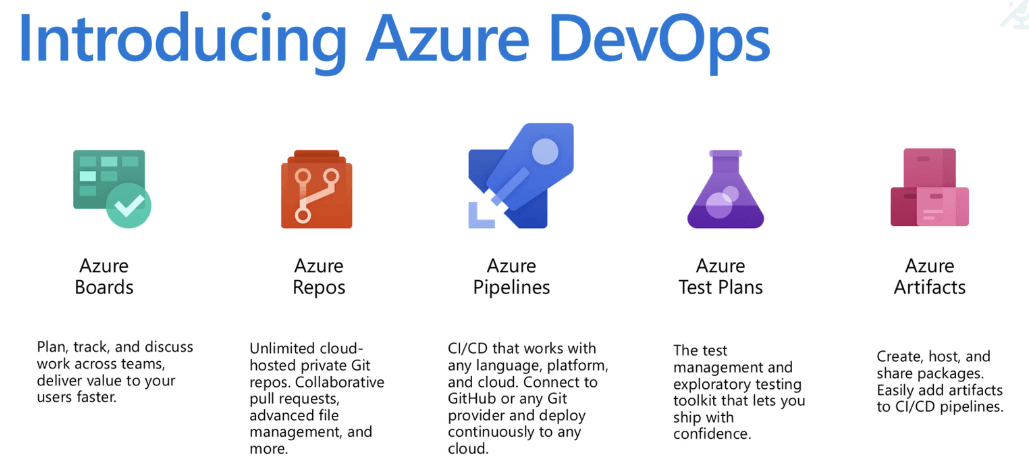
\includegraphics[scale=0.4]{img/azure.png}
    \caption{Azure DevOps, la solution de gestion de projet agile de Microsoft}
    \label{fig:my_label}
\end{figure}

C'est une plateforme très complète qui permet même d'associer à chaque \textbf{task}\footnote{Tâche en français. Fonctionnalité à implémenter/bug à résoudre dans le code} une \textbf{branche}\footnote{Une branche est une “copie" du code existant ; en réalisant une branche pour coder une nouvelle fonctionnalité il est facile de revenir en arrière en cas de problème} GitHub. De cette manière, le product owner n'a qu'à se charger de remplir le backlog avec l'ensemble des \textbf{user stories} et les tâches les composants ; puis l'équipe de développement créera une nouvelle branche de développement pour chacune de ces tâches. Lorsque le travail est terminé, la personne en charge du développement passe le code en validation (on appelle cela la \textbf{pull request}) ; de cette manière, le code est relu par les autres développeurs (dans notre cas, l'autre développeur), pour y déceler de possibles erreurs. Si les \textbf{reviewers} valident la modification, alors le nouveau code est ajouté au code pré-existant, sinon, le code est modifié jusqu'à entrer dans les critères.\\

\hfill \\
Si \textbf{Azure DevOps} était notre outil de gestion de projet par excellence, nous avions besoin d'un outil pour communiquer entre membres de l'équipe. Nous avons arrêté notre choix sur \textbf{Slack}\\

\begin{figure}[!h]
    \centering
    
\includegraphics[scale=0.15]{img/slack.png}
    \caption{Slack, notre outil de communication interne}
    \label{fig:my_label}
\end{figure}

Slack facilite la communication entre équipes grâce à l'utilisation de canaux de discussion distincts en fonction du rôle de chacun au sein du projet. Ainsi, les non-développeurs n'ont pas besoin d'avoir accès aux canaux réservés au développement d'application tout comme seuls les membres du service comptabilité accéderont au canal qui leur est réservé.\\

Dans notre cas, M. \textsc{Lecointre} et Mme. \textsc{Oudard} n'avaient aucun intérêt à avoir les messages réservés au développement, cependant il était pratique d'avoir un canal dédié pour communiquer avec eux dans le cas où nous avions des questions à leur poser. M. \textsc{Albers} était évidemment lui aussi présent sur le \textbf{Slack} de manière à l'inclure dans notre projet et faciliter les préparations de réunion.\\

\begin{figure}[!h]
    \centering
    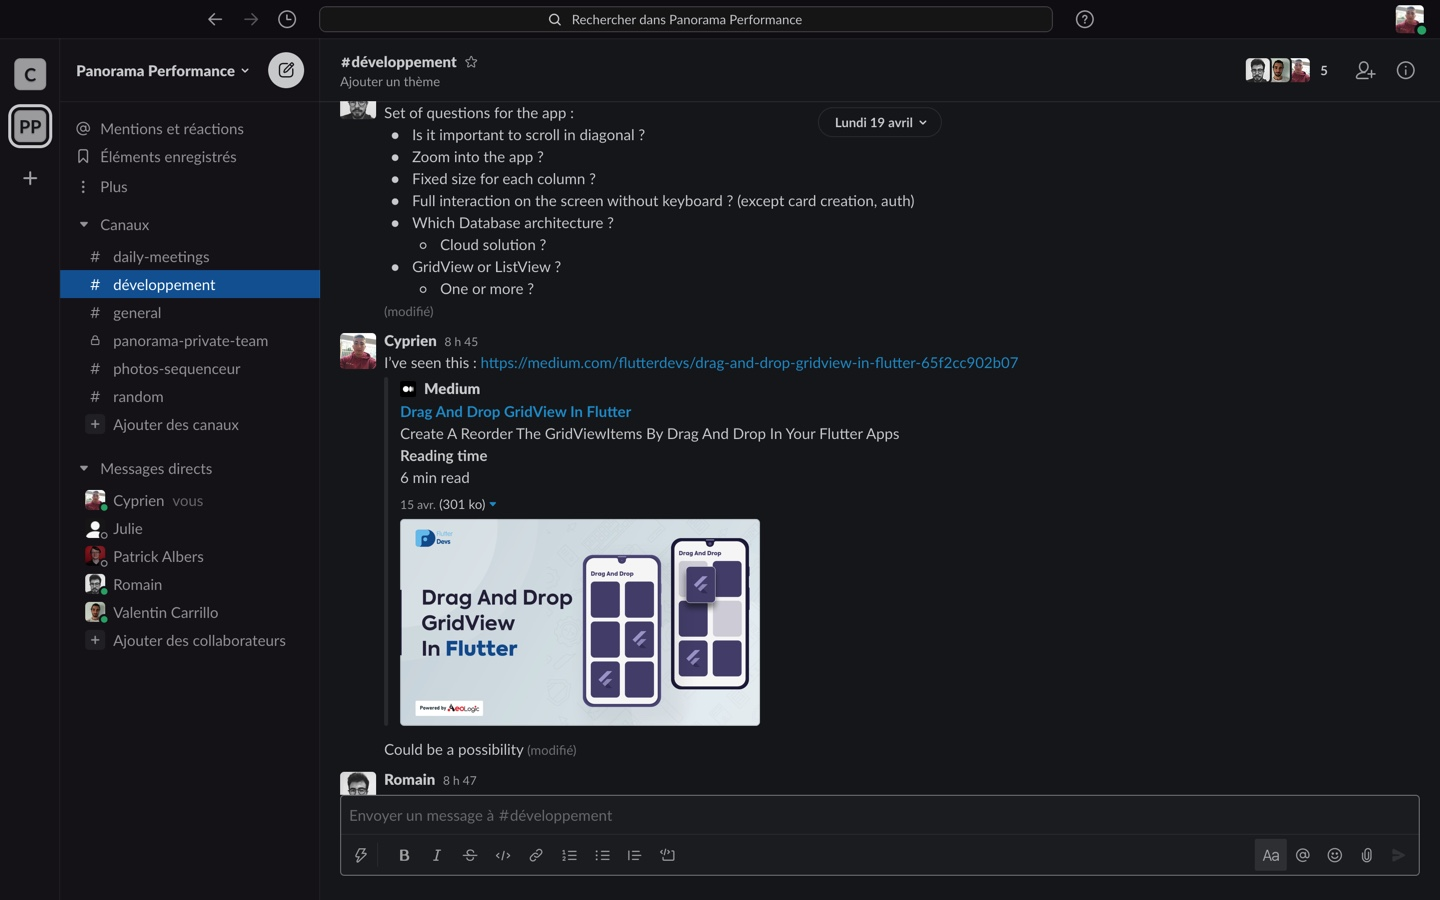
\includegraphics[scale=0.3]{img/screen_slack.jpeg}
    \caption{Le canal développement où nous discutions des choix techniques}
    \label{fig:my_label}
\end{figure}


Chaque daily meeting que nous avions tous les trois organisé était par exemple accessible par tous sur le canal \texttt{\#daily-meetings} sous forme d'un compte-rendu de réunion pdf.\\

Enfin, notre dernier outil de communication a été \textbf{Microsoft Teams}. Nous nous en sommes servis pour réaliser nos réunions avec M. Albers, tuteur au sein de l'ESAIP. Comme il nous est difficile de nous déplacer en ces temps de Covid, il nous a semblé préférable de réaliser les réunions d'avancement en visioconférence, et pour cela, Microsoft Teams est un outil fiable et nous permettant de partager nos écrans.

\begin{figure}[!h]
    \centering
    
\includegraphics[scale=0.2]{img/teams.jpg}
    \caption{Microsoft Teams, notre outil de visioconférence}
    \label{fig:my_label}
\end{figure}

\subsubsection*{Pair Programming}
\addcontentsline{toc}{subsubsection}{Pair Programming}

Pour ce qui est de la partie programmation, nous avons voulu profiter de cette expérience en entreprise pour tenter un nouveau type de méthodologie de travail : \textbf{le pair programming}\cite{PairProgrammingCodementor}.\\

La technique de pair programming fonctionne de la manière suivante : un des deux développeurs écrit le code tout en l'expliquant, le second peut à tout moment proposer des améliorations ou sa vision du code. Au bout d'une vingtaine de minutes, les développeurs échangent de place pour que tout deux passent un temps égal devant le clavier. Le développeur qui n'est pas devant le clavier décide de l'axe directeur du code, quoi faire en premier, et quelles seront les étapes suivante\footnote{Bien évidemment, l'avis du second développeur est pris en compte, mais s'il faut trancher, ce n'est pas lui qui tranchera.}, un peu comme un copilote qui s'occuperait du GPS (voir figure \ref{fig:PairProgramming} ci-dessous)\\


\begin{figure}[h!]
    \centering
    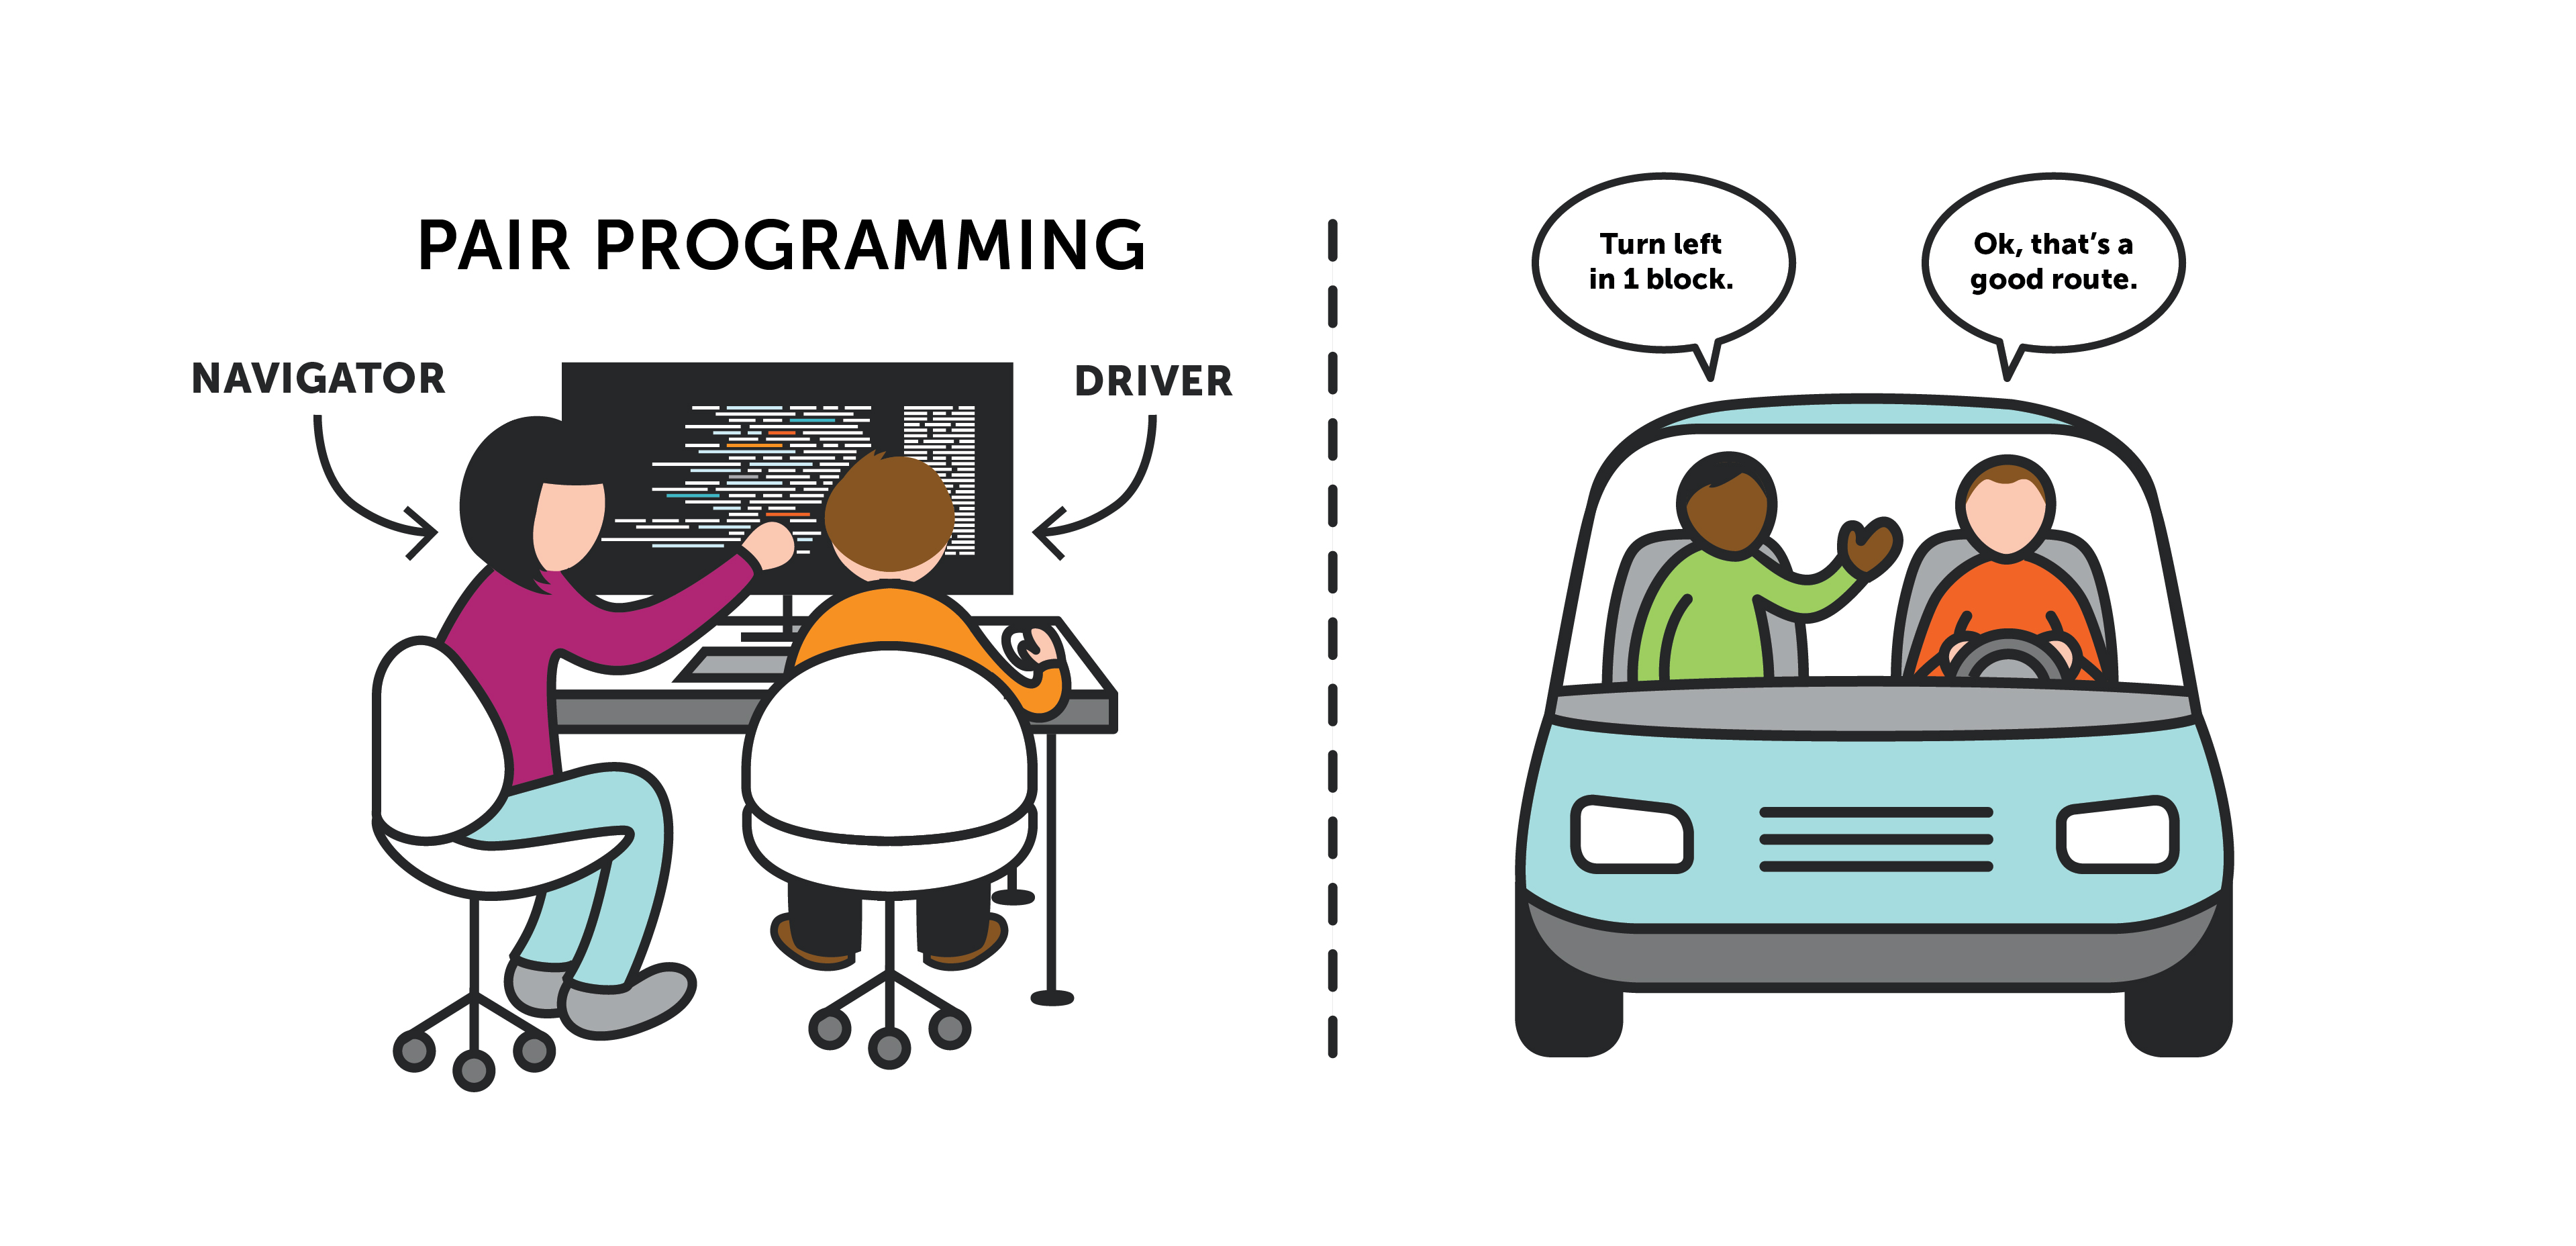
\includegraphics[scale=0.5]{img/pairprog.jpg}
    \caption{Le “pair programming", une technique de développement agile.}
    \label{fig:PairProgramming}
\end{figure}

L'intérêt d'une telle méthode est de produire un code de meilleure qualité en faisant travailler deux développeurs côte à côte ; de cette manière, deux approches sont confrontées dès la création du code et pas seulement dans la phase de debugging. La technique du pair programming est encore plus intéressante si l'on paire un développeur "senior" avec un "junior"\footnote{Entendre par là un développeur expérimenté dans le langage et un débutant}\\

Même si au premier abord, cette stratégie parait une perte de temps (deux fois moins de développeurs devant un clavier = deux fois moins de code, non ?), il n'en est en fait rien ! En effet, la partie gourmande en temps dans le développement d'applications est la réflexion ; écrire le code est très rapide une fois que les idées et la structure sont présents\footnote{Surtout de nos jours avec l'aide de \textbf{snippets} (auto-compléteur de code)}. Développer à deux permet d'éviter les erreurs d'étourderie ou les fausses bonnes idées, et ainsi gagner du temps de débugging. De plus, lorsque l'on travaille à deux, il y a une volonté de ne pas décevoir l'autre : on évite les distractions, les appels téléphoniques, on tape vite au clavier,\dots~Il y a quelqu'un pour nous aider à rester concentrés, ou lorsque l'on bute sur un problème de programmation. Enfin, d'après une étude menée en 2000, 96\% des développeurs ayant participé ont répondu mieux s'amuser lors du pair programming, et 95\% qu'il avaient plus confiance en leur code !~\cite{Williams00strengtheningthe}

\subsubsection*{Difficultés rencontrées et points d'améliorations}
\addcontentsline{toc}{subsubsection}{Difficultés rencontrées et points d'améliorations}

Bien que ce projet ne soit pas notre premier en terme de management de projet agile, nous sommes encore inexpérimentés sur certains concepts, et il nous arrive de ne pas respecter la mentalité \textsc{scrum} au pied de la lettre.\\

Ainsi, il n'était pas rare que la charge de travail que nous avions prévu lors du sprint planning ne soit pas suffisante, ou au contraire trop importante. Cela découle peut-être du fait que nous n'utilisions pas d'\textbf{indicateurs de performance} lors de notre projet. Il nous était donc impossible de calculer notre \textbf{vélocité}\footnote{En \textsc{scrum}, la vélocité est la charge de travail (en heure) que peut endurer l'équipe en un sprint.} ou d'afficher un \textbf{burndown chart}\footnote{Le burdown chart est un graphique affichant le nombre d'user stories en cours ou terminées ainsi que celles qui ont été créées durant le sprint} de qualité (voir figure \ref{fig:burndownChart}).\\

\begin{figure}[!h]
    \centering
    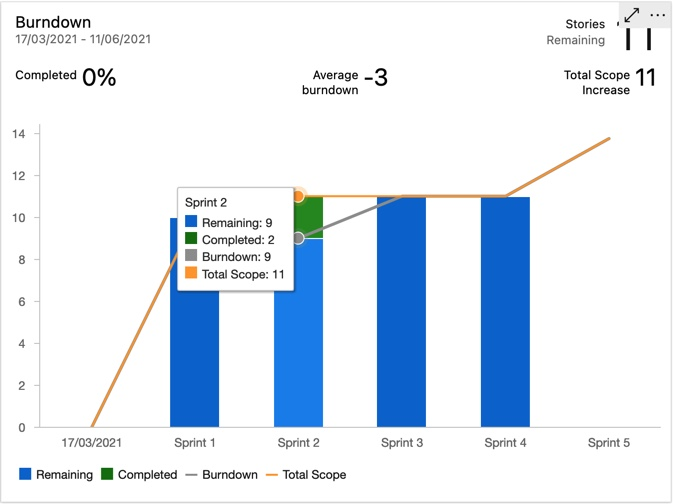
\includegraphics[scale=0.5]{img/burndown.jpeg}
    \caption{Le burdown chart}
    \label{fig:burndownChart}
\end{figure}

Pour combler le manque de charge de travail sur un sprint, nous étions dans l'obligation de modifier le sprint backlog, ce qui implique de rajouter des tâche au sprint en cours. Certes la team de développeurs se retrouvait avec du travail à réaliser, mais en contrepartie, il nous est arrivé de finir un sprint avec plus de travail à réaliser qu'à son début\footnote{Ce qui explique un burndown moyen négatif et une augmentation du scope\dots }

La taille de notre équipe est également un facteur négatif, la méthodologie \textsc{scrum} est plus complexe à mettre en place au sein de petites équipes, car le scrum master et/ou le product owner doivent alors doubler leur rôle en étant développeurs en même temps.\\

Mais il ne faut pas baisser les bras et rester agile ! Si ce projet n'a pas été mené à la perfection, les grandes lignes maîtresses du management agile ont été suivies et nous en avons beaucoup appris. À la manière agile, nous allons apprendre de nos erreurs et le prochain projet agile que nous mèneront n'en sera que meilleur.\\

Pour ce qui est du pair programming, cette première expérience s'avère concluante, même si toutes les directives n'ont pas étés tout le temps respectées à la règle. Par exemple, nous ne changions pas de rôle toutes les 20 minutes, ce qui provoqua un déséquilibre dans l'écriture de code que chacun de nous a réalisé. Cette pratique courante s'appelle \textbf{“Watch the Master"}\cite{enwiki:1023152145} et prend souvent place lorsqu'un développeur plus expérimenté prend place devant le clavier.



\subsection{Déroulement de la mission}

Pour mener à bien ce projet, nous avons décidé de suivre le calendrier suivant :
\begin{itemize}
    \item 1 semaine de recherche documentaire
    \item 3 semaines de développement de POC et de rédaction de rapport pour Panorama 
    \item 1 semaine de restitution à l'équipe de Panorama et de soutenance
\end{itemize}


\subsubsection*{Recherche Documentaire}
\addcontentsline{toc}{subsubsection}{Recherche Documentaire}

La première semaine de notre projet Activ'ESAIP nous a permis de nous familiariser avec le projet. Après une matinée de présentation de la mission par l'équipe de Panorama Performance, nous avons décidé de nous répartir les concepts importants qu'il nous fallait maîtriser pour sa réalisation, à savoir : 
\begin{itemize}
    \item M. \textsc{Girou} s'est occupé des recherches sur le concept de \textbf{Séquenceur}
    \item M. \textsc{Barbault} s'est chargé du \textbf{Lean Manufacturing}
    \item M. \textsc{Carrillo} a concentré ses recherches sur le \textbf{Management Visuel}
\end{itemize}

À la suite de cette semaine de recherches, nous avons chacun présenté le fruit de nos recherche et en avons ressorti des questions sur les points qui nous semblaient flous, de manière à pouvoir les poser à Mme. \textsc{Oudard} lors de la réunion que nous avions planifié le $1^{er}$ avril.\\

Nous avons également ressorti de cette première semaine le support le plus adapté pour garder l'aspect interactif de la solution, qui repose beaucoup sur le toucher. Notre première idée était de proposer un écran tactile de grande envergure, mais ce support s'avère très onéreux, donc peu accessible pour des PME et TPE. Nous avons donc arrêté notre choix sur un vidéo projecteur interactif comme ceux disponibles à l'ESAIP. 

\subsubsection*{Développement de la POC}
\addcontentsline{toc}{subsubsection}{Développement de la POC}

\begin{figure}[!h]
    \centering
    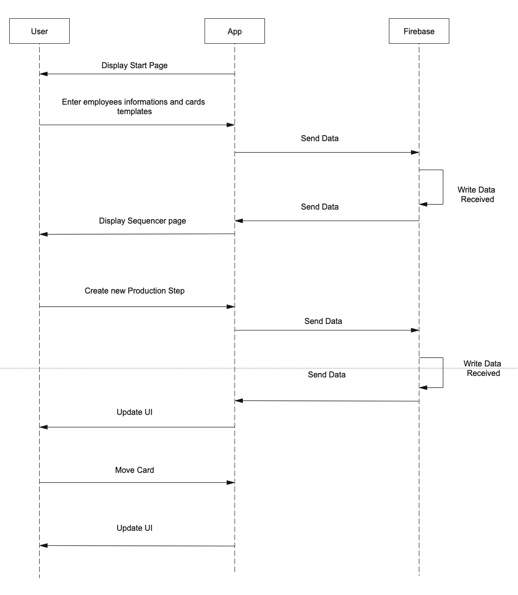
\includegraphics[scale=1]{img/sequence.jpeg}
    \caption{Le diagramme de séquence de l'application}
    \label{fig:POC}
\end{figure}


Durant les 3 sprints, respectivement du 19 au 23 avril, du 17 au 21 mai et du 31 mai au 4 juin, nous avons consacré nos efforts sur le développement d'une POC fonctionnelle.\\

Lors de la première semaine de développement, nous avons réussi à présenter à Panorama Performance une première version avec un tableau à double entrée présentant les deadlines de produit ainsi qu'un calendrier. Les “item\_production" (cf. figure \ref{fig:appV1}) pouvaient être stockés sur la base de données Firebase et l'application était déjà scrollable\footnote{Comprendre par ici que l'on peut faire défiler les lignes et colonnes à l'aide de la souris} selon les deux axes.\\


\clearpage


\begin{figure}[!h]
    \centering
    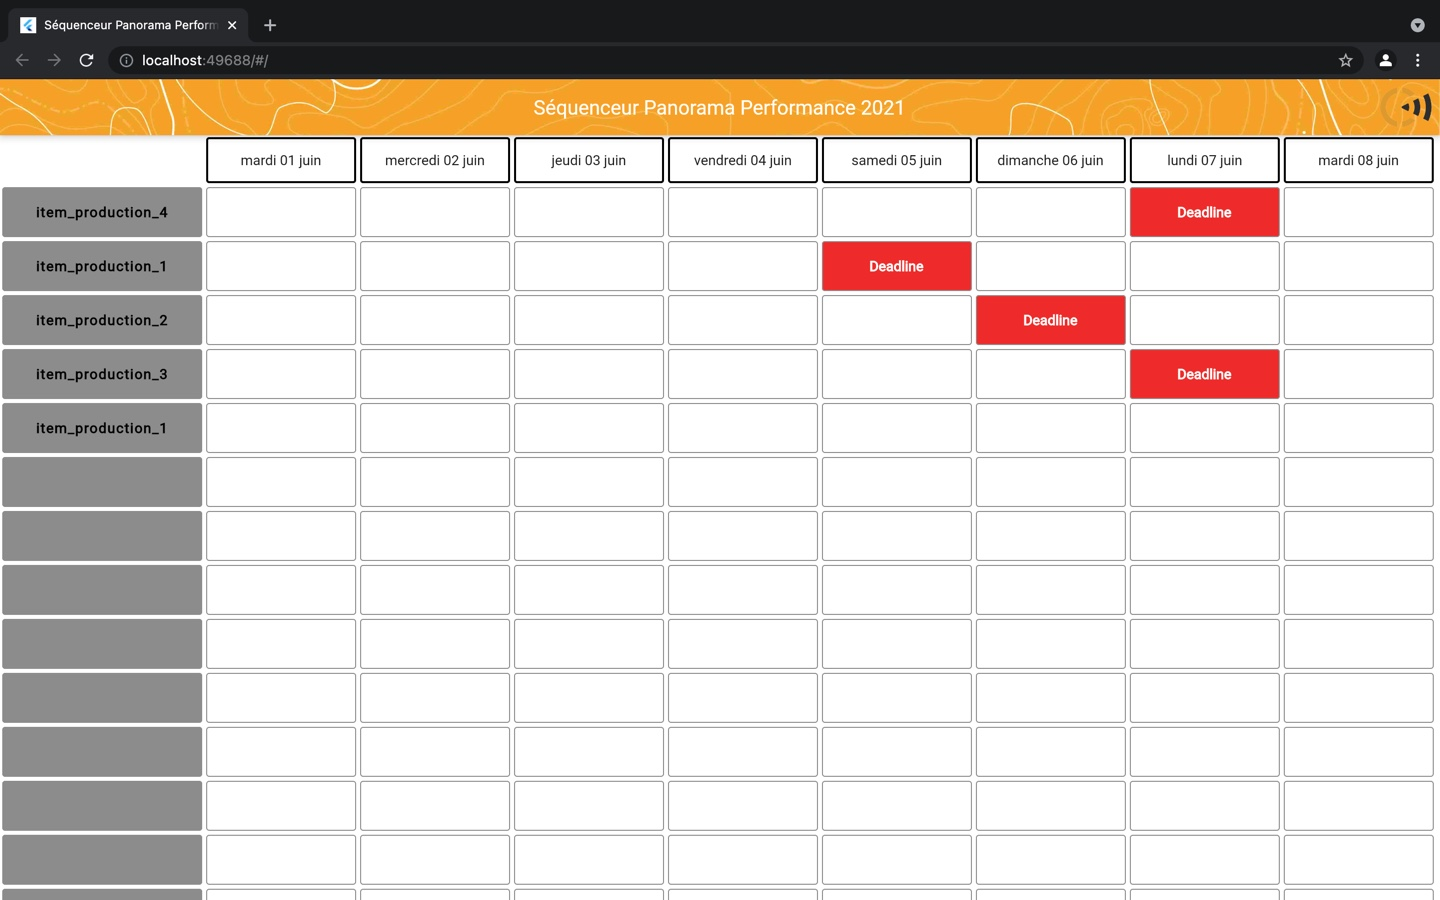
\includegraphics[scale=0.28]{img/app_v1.jpeg}
    \caption{Visuel de l'application après une semaine de développement}
    \label{fig:appV1}
\end{figure}

Nous avons également eu le temps de réaliser une page d'accueil qui permet à la fois la création de modèles pour les cartes (qui serviront à remplir la grille plus tard), ainsi que celle des différents salariés de l'entreprise et la tâche à laquelle ils peuvent être assignés. La page d'accueil est également munie de validators qui vérifient les différentes valeurs fournies par l'utilisateur avant de les écrire dans la base de données\footnote{Visible en rouge sur la figure \ref{fig:appV1StartPage}}.

\begin{figure}[!h]
    \centering
    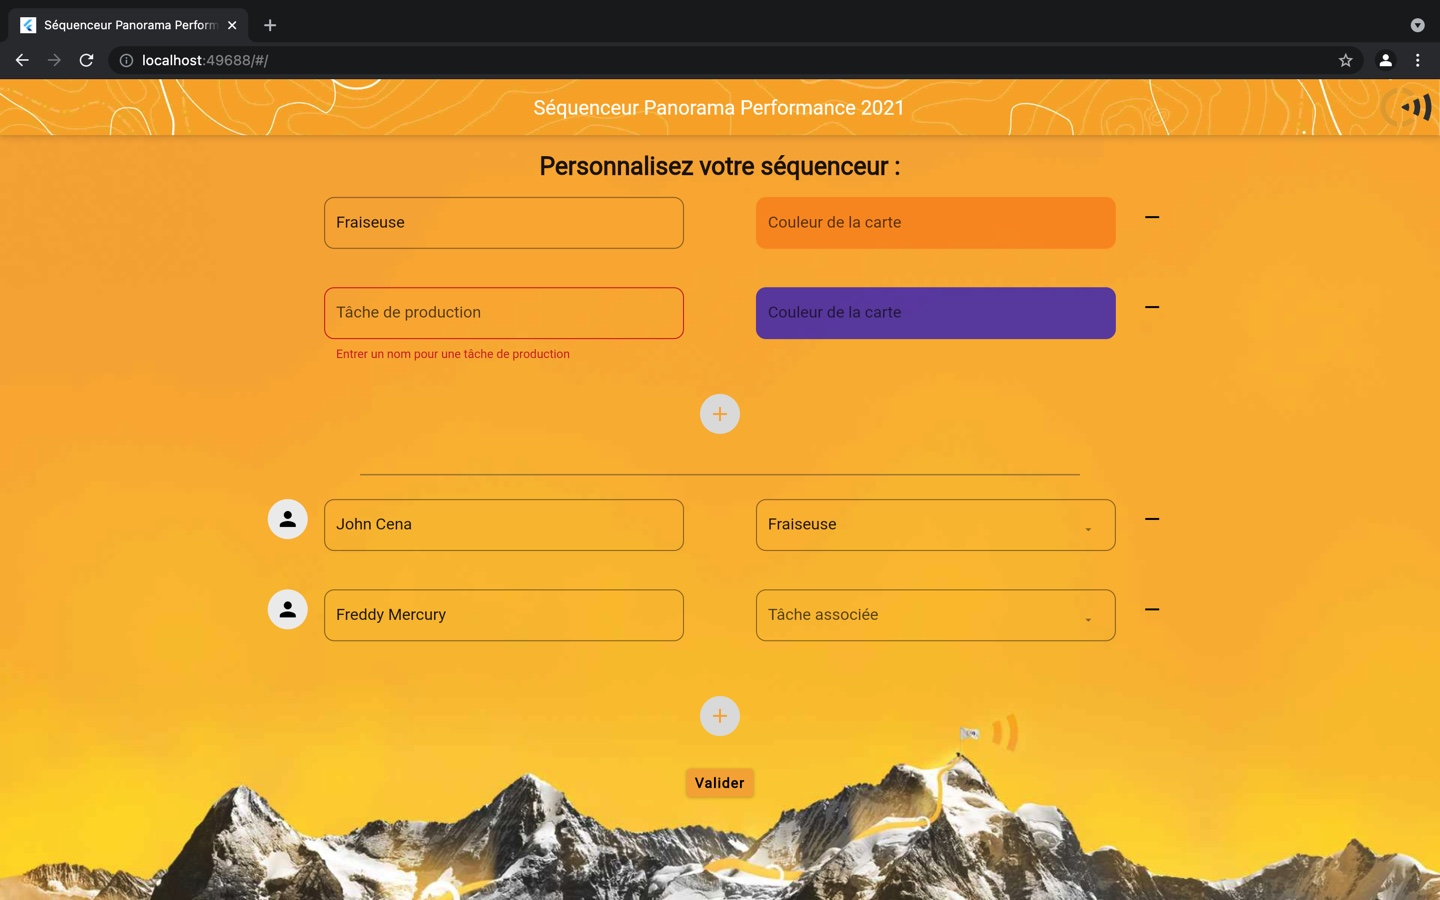
\includegraphics[scale=0.28]{img/app_v1_startPage.jpeg}
    \caption{La page d'accueil de l'application}
    \label{fig:appV1StartPage}
\end{figure}
\clearpage

L'objectif de la deuxième semaine a été de permettre la création d'étapes de production et de les récupérer pour les afficher dans la ligne qui leur correspondait.\\

Nous avons eu quelques difficultés à récupérer toutes les étapes correspondantes à une ligne de production, en effet comme vous pouvez le voir sur la figure \ref{fig:appV2}, les lignes possédant plusieurs étapes affichaient des erreurs. Cependant, la version que nous avons rendue à la fin de sprint offrait tout de même la possibilité de créer de nouvelles étapes de productions en tapotant sur une case vide d'une ligne munie d'un item de production. 


\begin{figure}[!h]
    \centering
    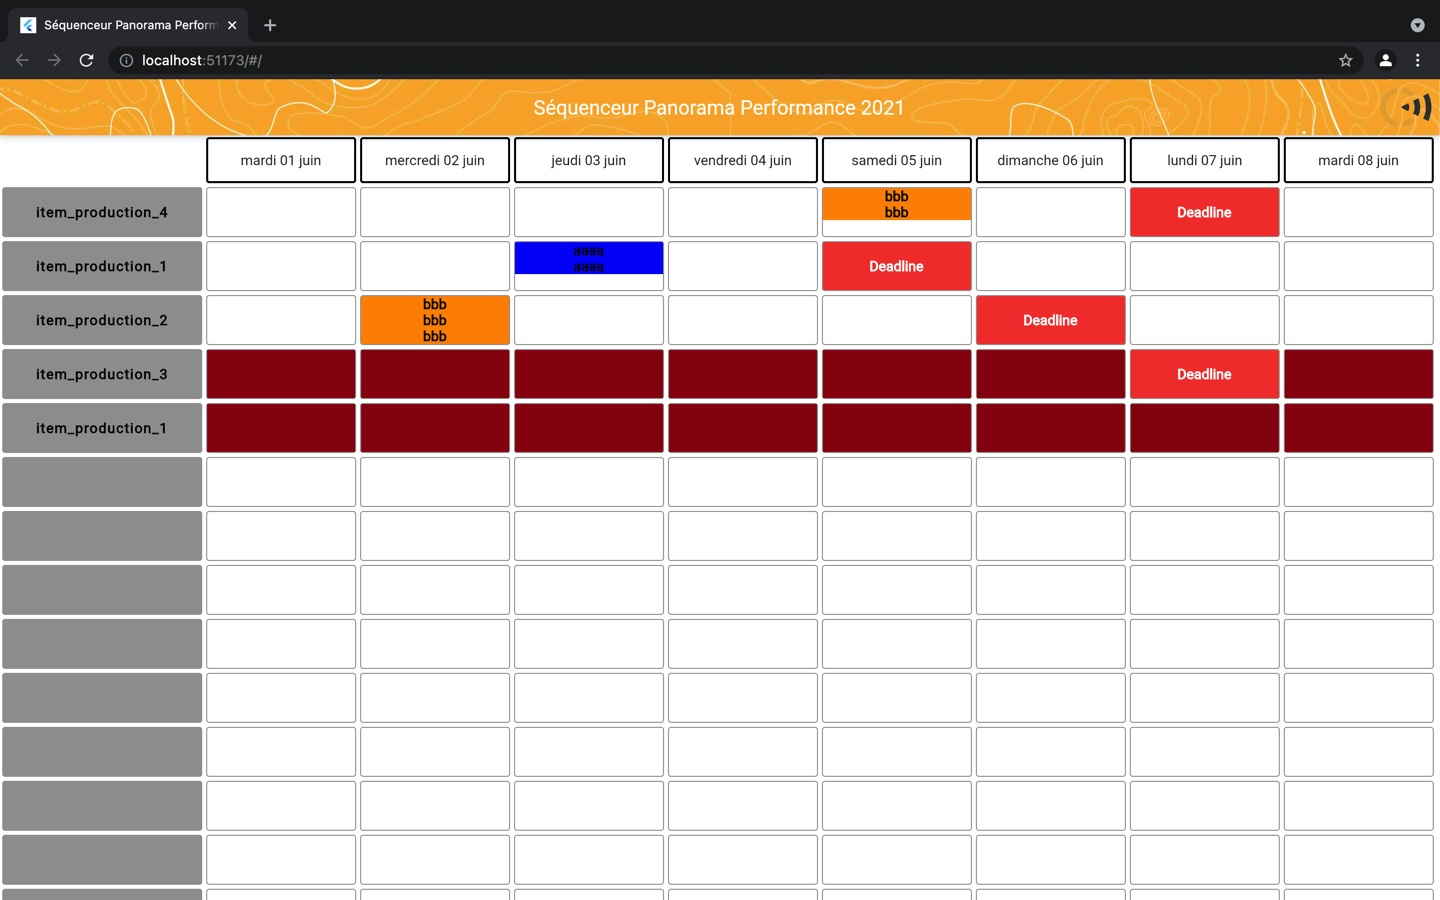
\includegraphics[scale=0.28]{img/app_v2.jpeg}
    \caption{Visuel de l'application à la fin du deuxième sprint}
    \label{fig:appV2}
\end{figure}

\begin{figure}[!h]
    \centering
    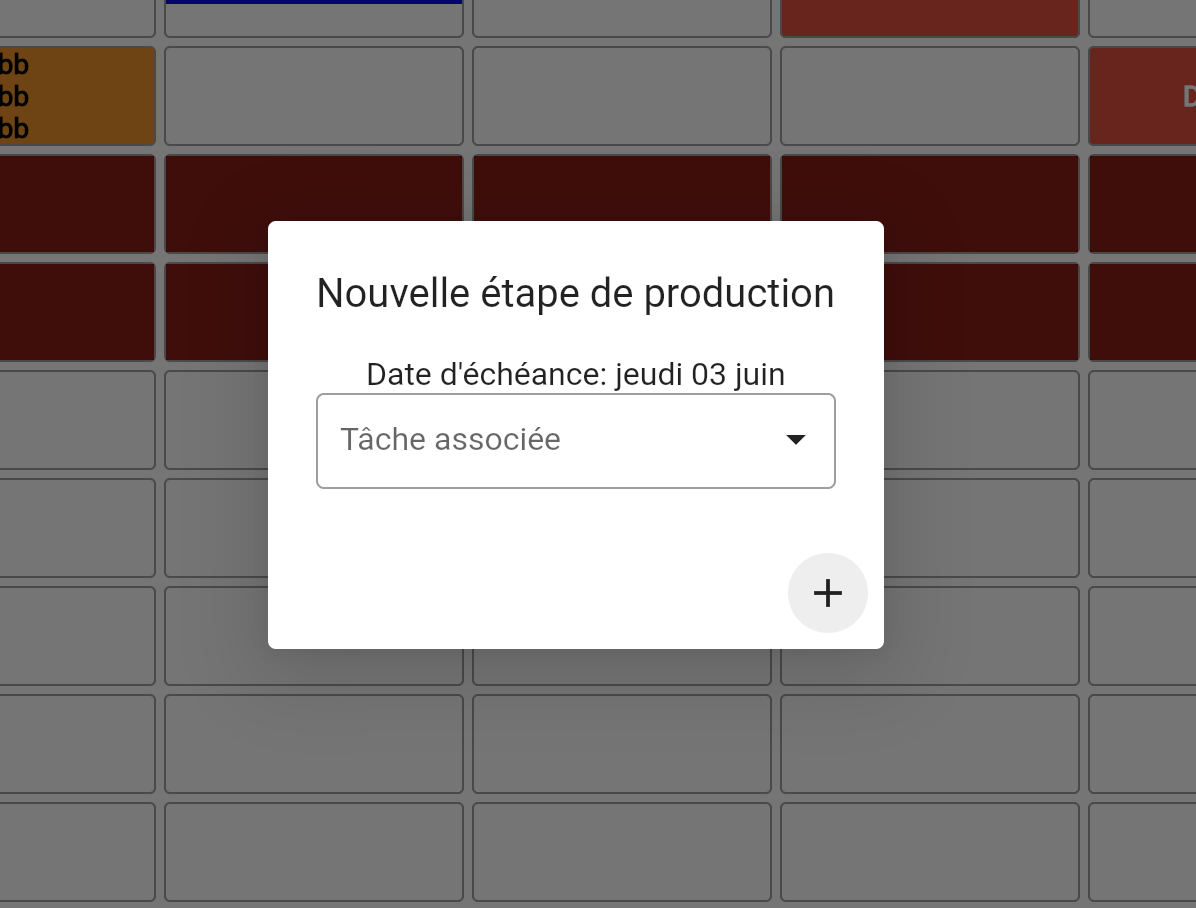
\includegraphics[scale=0.28]{img/creation_step.png}
    \caption{Fenêtre de création d'étape de production}
    \label{fig:creationStep}
\end{figure}

Nous avons également créé le formulaire de création d'items de production \footnote{correspondant à une ligne} et d'étapes de production \footnote{correspondant à une case} (voir figure \ref{fig:creationStep}). qui offre la possibilité de choisir une compétence parmi celles entrées dans la page de personnalisation du séquenceur (voir figure \ref{fig:appV1StartPage}). Les étapes apparaissent ensuite de la couleur choisie dans la ligne qui leur correspond.
\clearpage

Nous avions conclu avec Panorama Performance que la POC serait prête pour la fin du $3^{e}$ sprint, mais pour coller avec leurs disponibilités, nous avons dû avancer la date au mercredi 2 juin. Ainsi, la version que nous leur avons présentée n'était pas exempte de bugs, mais elle était belle et bien fonctionnelle.


\begin{figure}[!h]
    \centering
    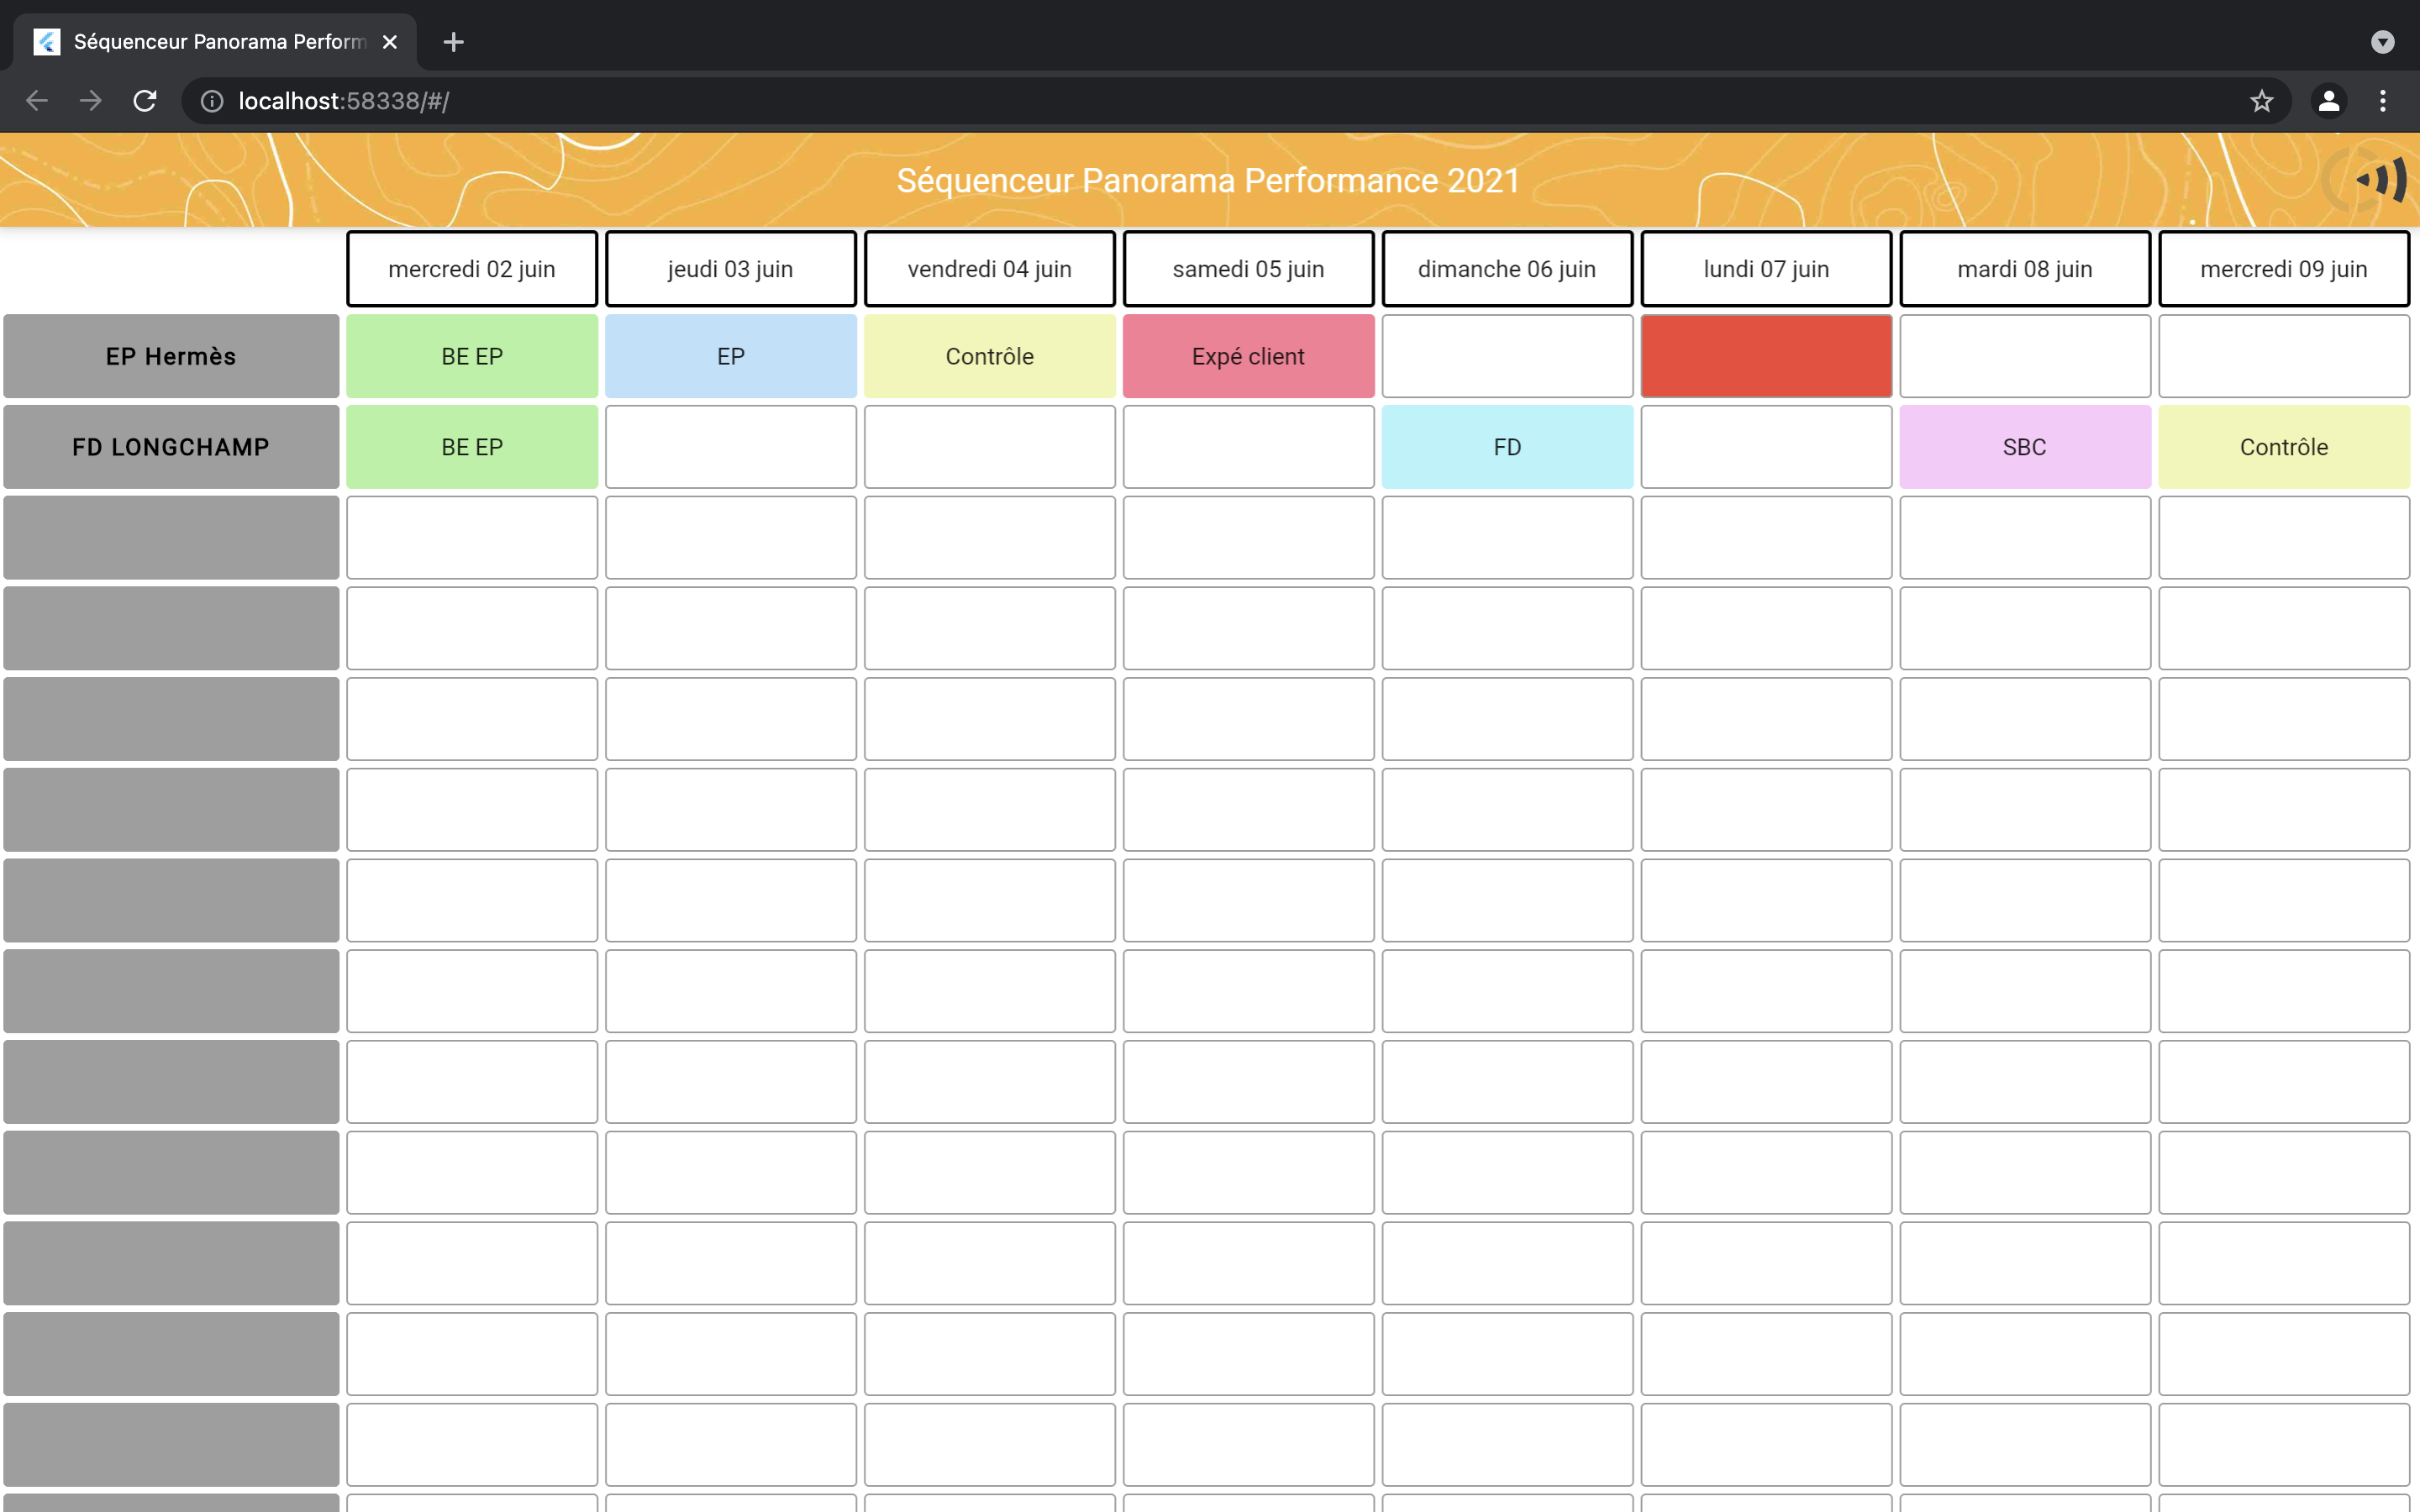
\includegraphics[scale=0.28]{img/app_v3.png}
    \caption{Visuel de la POC telle qu'est sera rendue à Panorama Performance}
    \label{fig:POC}
\end{figure}


Comme vous pouvez le voir ci-dessus, dans la figure \ref{fig:POC}, la POC est une version plus complète que les versions précédentes. Nous avons eu le temps d'y ajouter le déplacement des cartes d'étapes de production. Cela offre la possibilité de ré-arranger leur ordre ou changer leur date d'exécution.\\
\hfill

La $3^{e}$ semaine de développement à également été l'occasion de présenter notre POC à l'équipe de Panorama Performance. Nous voulions leur présenter une application fonctionnelle pour qu'ils aient la possibilité de l'essayer en s'appuyant sur un cas réel. L'essai s'est très bien déroulé et M. \textsc{Lecointre} et Mme. \textsc{Oudard} se sont avérés agréablement surpris par la facilité d'utilisation de l'application.\\

Le test s'étant déroulé dans la salle \textbf{E004} de l'ESAIP, nous avons eu la chance pouvoir utiliser le \textbf{VPI} pour présenter l'application dans un contexte réel d'utilisation. L'application s'est avérée très simple à utiliser avec les stylos “tactiles" du VPI, et la taille d'écran a parue satisfaisante pour remplacer la solution actuelle. La manière dont nous avons désigné la création et le déplacement de carte a aussi plu à Panorama Performance : plus contraignante que la version papier, elle obligerait ainsi les entreprises à utiliser les flux tirés\footnote{Certaines méthodologies des flux tirés sont peu naturelles à mettre en place (ne pas faire tourner les machines en permanence à plein régime, se plier au rythme du poste le plus lent, \dots )}




\subsubsection*{Rédaction du rapport de faisabilité}
\addcontentsline{toc}{subsubsection}{Rédaction du rapport de faisabilité}


\todo{À faire par Valentin ??}


\section{Partie Financière}

Lors du projet Activ'ESAIP, l'équipe d'étudiant vient se substituer à une équipe d'ingénieurs de conseil. C'est un dispositif intéressant pour l'entreprise car bien moins coûteux !\\

Il est intéressant d'estimer les gains réalisés par l'entreprise en choisissant le dispositif Activ'ESAIP, et c'est ce que nous allons estimer au cours de cette partie financière.

\subsection{Coût de l'Activ'ESAIP pour l'entreprise}

Lors de cette mission, trois étudiants ingénieurs ont été mobilisés par Panorama Performance : deux étudiants en Informatique et Réseaux et un étudiant en Sécurité, Environnement et Prévention des risques. Selon la grille tarifaire de l'ESAIP\footnote{Voir Annexe A}, cela correspond à une facture de 2550\euro. Cette somme est \textbf{TTC} car Panorama Performance ne récupère pas de \textbf{TVA}.\\

L'entreprise n'a pas eu de frais de déplacement supplémentaire à payer, car nous résidons tous les trois sur Angers. Bien que M. \textsc{Lecointre} soit légalement notre tuteur entreprise, c'est Mme. \textsc{Oudard} qui s'est chargée de nous encadrer et de répondre à nos questions en cas d'interrogations. Pour autant, nous avons su faire preuve d'autonomie sur une grande majorité du projet, ce qui a permis à l'équipe de Panorama Performance d'éviter des coûts indirects en consacrant du temps, normalement réservé à leurs clients, à ce projet. 

\subsection{Estimation des coûts réels de la mission}

Pour rappel, nous avons décidé de diviser nos 5 semaines en : 
\begin{itemize}
    \item Une semaine de recherche
    \item 3 semaines de développement et de rédaction d'un business model
    \item Une semaine de bilan entreprise et soutenance
\end{itemize}
L'équipe de Panorama Performance ne possédant pas de profil \textbf{IT}, il y aurait donc eu une obligation de faire appel à un tiers. Nous avons donc décidé de faire plusieurs hypothèses en appliquant les tarifs \textbf{free-lance} disponibles en lignes \cite{SalaireFreeLance}. Nos calculs sont basés sur une semaine d'étude de faisabilité et 3 semaines de développement (la $5^{e}$ n'est pas comptée car pas immédiatement reliée au projet).\\

En prenant un salaire moyen journalier de 500\euro/jour pour le développement de l'application, et de 400\euro/jour pour l'étude de faisabilité du projet, nous avons estimé un coût total pour le projet de 25.334\euro~HT.
\clearpage

\begin{figure}[!h]
    \centering
    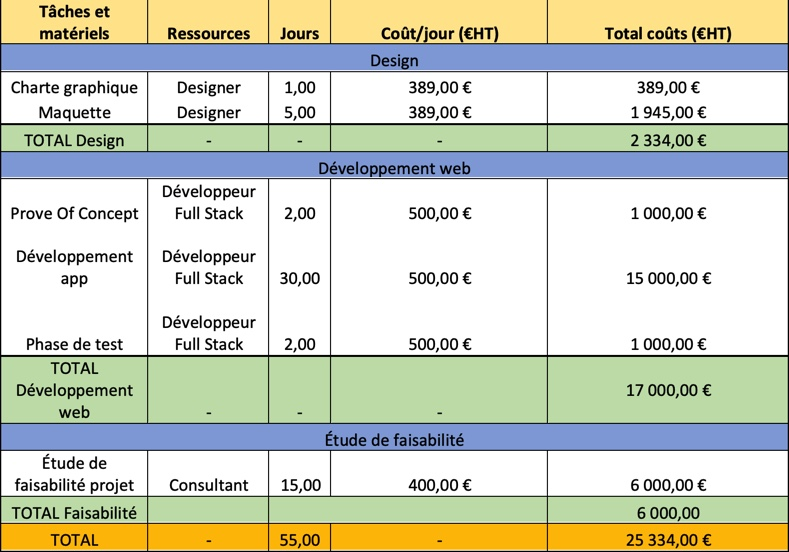
\includegraphics[scale=0.5]{img/estimation_prix_poc.jpeg}
    \caption{Tableau estimatif des coûts de développement d'une POC}
    \label{fig:TabEstimationPOC}
\end{figure}

Rappelons que ces estimations sont réalisées dans le cadre du développement d'une POC et non pas de l'application finale de séquenceur attendue par Panorama Performance. Pour une telle tâche, un travail de 5 semaines minimum sur le développement de la digitalisation du séquenceur aurait été l’idéal en embauchant en Free-lance des développeurs Full Stack. 


\begin{figure}[!h]
    \centering
    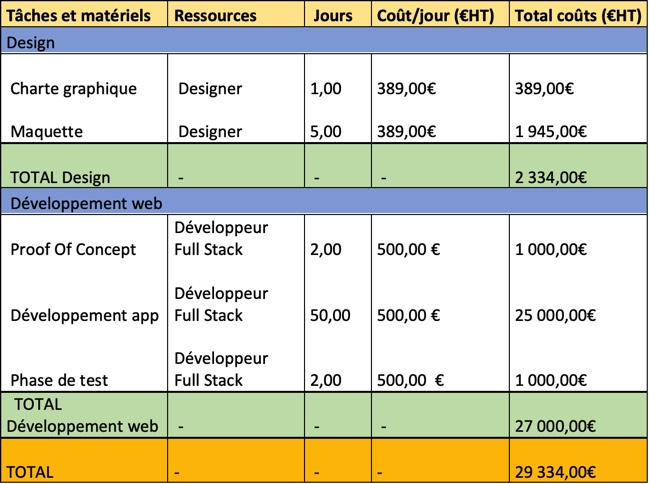
\includegraphics[scale=0.5]{img/estimation_prix_projetFL.jpeg}
    \caption{Tableau estimatif des coûts de développement de l'application finale}
    \label{fig:TabEstimationAppFL}
\end{figure}
\clearpage

Une autre option aurait été de travailler avec une entreprise de développeurs, ce qui permettra d’avoir un suivi régulier si des problèmes arrivent après le déploiement de la solution. Cette solution est bien évidemment plus onéreuse. On peut compter sur une moyenne de 800\euro~par jour pour chaque développeur. Cette option coûterait 45 534\euro~à Panorama Performance (voir ci-dessous Fig:  \ref{fig:TabEstimationAppDev}).


\begin{figure}[!h]
    \centering
    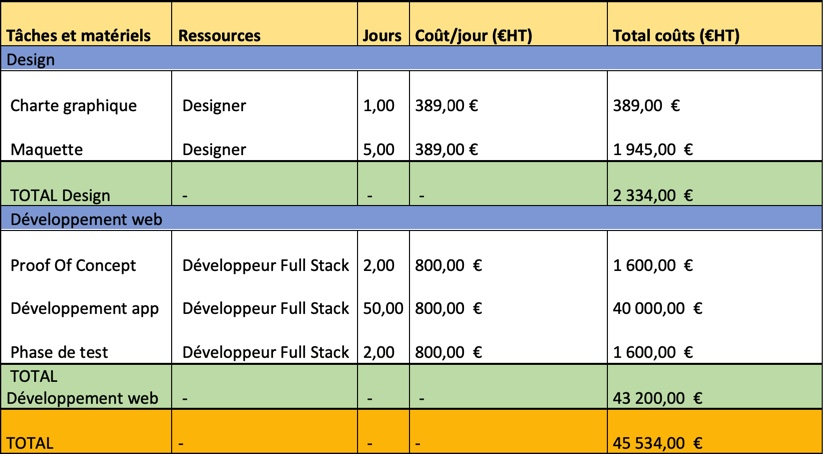
\includegraphics[scale=0.5]{img/estimation_prix_projetDev.jpeg}
    \caption{Tableau estimatif des coûts de développement de l'application finale par une entreprise de développement}
    \label{fig:TabEstimationAppDev}
\end{figure}


On peut donc en conclure que Panorama Performance sort gagnant de cette collaboration. En effet, ils auront, grâce à une somme dépensée de 2500\euro, bien inférieure à 10\% du coût final du projet, obtenu une version très poussée du séquenceur numérique ainsi qu’une étude de faisabilité de cette digitalisation.
\section{Résultats et livrables entreprise}
Comme les attentes initiales de Panorama Performance s’approchaient trop d’une application complète (plus que d’une POC) et que nous avions trop peu de temps pour développer toutes les fonctionnalités que l’équipe souhaitait, nous avons dû choisir un certain nombre de fonctionnalités à implémenter. Notre objectif était de développer une POC, la plus simple possible, mais munie des fonctionnalités principales, afin de voir si ce projet était réellement viable et pourrait être au minimum équivalent à la version papier. \\

Nous avons estimé les différentes options afin d’effectuer cette digitalisation, et nous avons retenu que la faire réaliser par un freelance était le plus rentable. Cependant, sur le long terme, il vaudrait mieux embaucher un développeur Full Stack au sein de l’entreprise afin de pouvoir améliorer la solution et corriger les éventuels problèmes.\\

Nous avons également réalisé une partie économique de ce projet afin de pouvoir voir si ce projet était rentable grâce à la création d’un abonnement annuel. Nous avons donc estimé que ce projet l’était, avec un retour sur investissement sur 3 ans après le déploiement de la solution.\\

 Suite à la phase de test réalisé le mercredi 2 juin en salle E004, Panorama Performance nous a annoncé vouloir pousser le développement pour obtenir un MVP. Ils présenteront ensuite l'application à leurs clients les plus réguliers, et en fonction de leurs retour (usabilité, simplicité, besoin, \dots) ils lanceront, ou non, le développement final.\\
 
 \begin{figure}[!h]
     \centering
     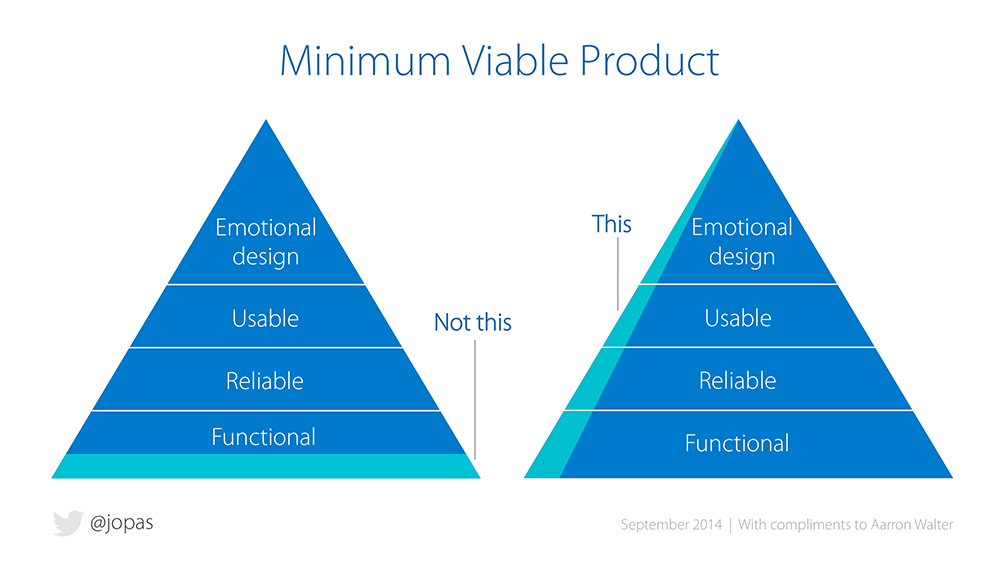
\includegraphics[scale=0.3]{img/MVP.png}
     \caption{Principe du Minimum Viable Product}
     \label{fig:my_label}
 \end{figure}

La dernière semaine du projet va également être l'occasion de commenter le code pour permettre sa transmission à une possible nouvelle équipe de développement. De cette manière, le projet n'aura pas à repartir de zéro. Le code ainsi que l'accès à la base de données seront en effet fournis à Panorama Performance à la fin de ce projet Activ'ESAIP, de cette manière, ils pourront présenter la version qui est déjà disponible en ligne, mais également en modifier certaines fonctionnalités ou en ajouter.
\section{Conclusion}
This applicative project and first part of the sigma racing was very interesting. \\
We learned a lot and we now know that we are really pasionate about image recognition and deep learning.\\

It is a very complex domain and we are far from mastering it. Nevertheless, we have done our best in order to make a working model. We took deep learning online classes and read books to complete our train. It seemed, at first, very complexe (mostly the mathematicals aspects, and its still is !) but we managed to understand the basics and we are learning more every days.\\

This project will come to an end on June 2021. The next step is to buy the car and implement all the work that we have done inside it. We also plan to design our own removable track with the same specifications as the official one in order to test the car in different track configurations. Moreover, we will need to get cracking on the obstacles detections (is a Lidar sensor usefull ?) as well as the start and finish behaviors of the car.\\

We are still struggling with the hardware as we cannot borrow a GPU for the schools servers. It has a direct affect on the duration of the training and some help in this area would be more than welcome.

\hfill \\ 

\begin{figure}[!h]
\centering

\includegraphics[scale=0.15]{img/girou_barbault.jpg}
\caption{Romain (left) and Cyprien (right)}
\end{figure}
\clearpage
\section{Bilans personnels}
\subsection*{Romain}
\addcontentsline{toc}{subsection}{Romain}

Je me suis concentré principalement sur le développement d’une POC durant ce projet Activ’esaip. Comme chaque projet de développement, l’élément clé est la définition des objectifs. Panorama Performance n’avait pas une idée claire de ce qu’ils souhaitaient développer en début de projet. C’est pourquoi il nous a fallu redéfinir les objectifs à la fin de la deuxième semaine. Cette redéfinition, plus réaliste et faisable, nous a permis de nous concentrer sur les fonctionnalités principales et essentielles à Panorama Performance.\\

Le développement a été en lui même un défi de taille. Cette notion de “simplexité”\footnote{La simplexité est l’art de rendre simples, lisibles, compréhensibles les choses complexes. C'est une notion émergente et un domaine d'étude nouveau en systémique, ingénierie et neurosciences.} a guidée ma façon d’aborder le développement. Cependant, les applications en apparence simple abritent en réalité un code assez complexe. Cela aura donc été un challenge qui, selon moi, a su être relevé.
La solution développée est une application web développé sous Flutter, utilisant les services de Firebase pour le backend, notamment Cloud FireStore, la base de donnée NoSQL. \hfill \\

Globalement, ce projet a été très enrichissant, et ce, sur de nombreux aspects. Le plus important selon moi est la pleine considération de nos compétences et de notre réflexion. Panorama Performance nous a intégrés, depuis le début du projet, comme des ingénieurs. Les questions qui nous été posées n’étaient donc pas limitées à l’aspect technique. Dès lors, nous avons pu prendre pleinement conscience de la vision transversale qu’un ingénieur doit avoir. Nous devons être irréprochables techniquement, mais nous devons aussi être en capacité de réaliser des études de marchés, des business models, …

\subsection*{Cyprien}
\addcontentsline{toc}{subsection}{Cyprien}

Après 4 ans d'études à l'ESAIP et plus particulièrement 2 ans de cycle ingénieur, nous avons enfin été confrontés à un projet professionnalisant. Travailler au contact d'une entreprise ne peut pas être appris dans des livres et on ne peut pas prévoir comment réagir une fois jeté dans le monde réel. Je trouve particulièrement enrichissant d'avoir réalisé ce projet avec un ancien élève de l'école, cela prouve la porté du réseau des anciens.
\hfill \\

Tour à tour développeur et Scrum master, j'ai une fois de plus pu constater la force de la méthode de management agile, de l'amélioration et du retour client. Cela m'a conforté dans mon idée de me spécialiser dans le management d'équipe à moyen ou long terme car, j'aime cet aspect de la gestion de projet. Je n'en suis pas à mon premier projet en compagnie de Romain \textsc{Girou} et nous avons déjà nos routines de travail ; nous savons comment fonctionne l'autre et comment nous répartir les tâches pour que le projet avance au plus vite. C'était cependant la première fois que nous décidions de travailler en pair-programming, une technique intéressante si bien maîtrisé, je pense retenter l'expérience lors d'une prochaine mission si l'occasion se présente.
\hfill \\

Je trouve que Panorama Performance nous a accueilli comme les (futurs) ingénieurs que nous sommes, et nous a laissé carte blanche sur la gestion du projet tant que nous respections les dead-lines et les livrables. Ils nous ont même félicité pour notre autonomie et notre professionnalisme.
\hfill \\

Je retiendrais ce projet Activ'ESAIP comme une excellente expérience, qui m'aura initiés aux différents concepts de la performance industrielle, plus particulièrement au séquenceur et à la force de concepts comme les flux tirés ou de la production juste à temps. J'ai également pu perfectionner ma maîtrise de Flutter, et plus particulièrement au “state management" avec la méthodologie BLoC. Cela me sera très utile pour mon stage de cet été où je serais amené une fois de plus à développer en Flutter.


\clearpage
\section*{Liste des figures}
\addcontentsline{toc}{section}{Liste des figures}
\listoffigures

\clearpage
\section*{Bibliographie}
\addcontentsline{toc}{section}{Bibliographie}
\nocite{*}
\bibliographystyle{plain}
\bibliography{references}

\begin{appendices}
\subsection{Code for the Lane Detection algorithm}\label{laneDetect}
\begin{python}
import cv2
import numpy as np
 
def make_points(image, line):
    slope, intercept = line
    y1 = int(image.shape[0])# bottom of the image
    y2 = int(y1*3/5)         # slightly lower than the middle
    x1 = int((y1 - intercept)/slope)
    x2 = int((y2 - intercept)/slope)
    return [[x1, y1, x2, y2]]
 
def average_slope_intercept(image, lines):
    left_fit    = []
    right_fit   = []
    if lines is None:
        return None
    for line in lines:
        for x1, y1, x2, y2 in line:
            fit = np.polyfit((x1,x2), (y1,y2), 1)
            slope = fit[0]
            intercept = fit[1]
            if slope < 0: # y is reversed in image
                left_fit.append((slope, intercept))
            else:
                right_fit.append((slope, intercept))
    # add more weight to longer lines

    if len(left_fit) and len(right_fit):
    #over-simplified if statement (should give you an idea of why the error occurs)
       left_fit_average  = np.average(left_fit, axis=0)
       right_fit_average = np.average(right_fit, axis=0)
       left_line  = make_points(image, left_fit_average)
       right_line = make_points(image, right_fit_average)
       averaged_lines = [left_line, right_line]
       return averaged_lines
 
def canny(img):
    gray = cv2.cvtColor(img, cv2.COLOR_RGB2GRAY)
    kernel = 5
    blur = cv2.GaussianBlur(gray,(kernel, kernel),0)
    canny = cv2.Canny(gray, 50, 150)
    return canny
 
def display_lines(img,lines):
    line_image = np.zeros_like(img)
    if lines is not None:
        for line in lines:
            for x1, y1, x2, y2 in line:
                cv2.line(line_image,(x1,y1),(x2,y2),(0,255,0),10)
    return line_image
 
def region_of_interest(canny):
    height = canny.shape[0]
    width = canny.shape[1]
    mask = np.zeros_like(canny)
 
    triangle = np.array([[
    (200, height),
    (550, 250),
    (1100, height),]], np.int32)
 
    cv2.fillPoly(mask, triangle, 255)
    masked_image = cv2.bitwise_and(canny, mask)
    return masked_image
 

# Code for the detection in an image named 'test_image.jpg'
image = cv2.imread('test_image.jpg')
lane_image = np.copy(image)
lane_canny = canny(lane_image)
cropped_canny = region_of_interest(lane_canny)
lines = cv2.HoughLinesP(cropped_canny, 2, np.pi/180, 100, np.array([]), minLineLength=40,maxLineGap=5)
averaged_lines = average_slope_intercept(image, lines)
line_image = display_lines(lane_image, averaged_lines)
combo_image = cv2.addWeighted(lane_image, 1, line_image, 1, 1)
cv2.imshow("result", combo_image)
cv2.waitKey(0)
cv2.destroyAllWindows()

# Code for the detection in a video named 'test2.mp4'
#cap = cv2.VideoCapture("test2.mp4")
#while(cap.isOpened()):
#    _, frame = cap.read()
#    canny_image = canny(frame)
#    cropped_canny = region_of_interest(canny_image)
#    lines = cv2.HoughLinesP(cropped_canny, 2, np.pi/180, 100, np.array([]), minLineLength=40,maxLineGap=5)
#    averaged_lines = average_slope_intercept(frame, lines)
#    line_image = display_lines(frame, averaged_lines)
#    combo_image = cv2.addWeighted(frame, 0.8, line_image, 1, 1)
#    cv2.imshow("result", combo_image)
#    if cv2.waitKey(1) & 0xFF == ord('q'):
#        break
#cap.release()
#cv2.destroyAllWindows()
\end{python}
\clearpage

\subsection{Image at each step in the lane detect algorithm}
\label{imagelaneDetect}
\begin{figure}[!h]
\begin{minipage}{7cm}
\centering
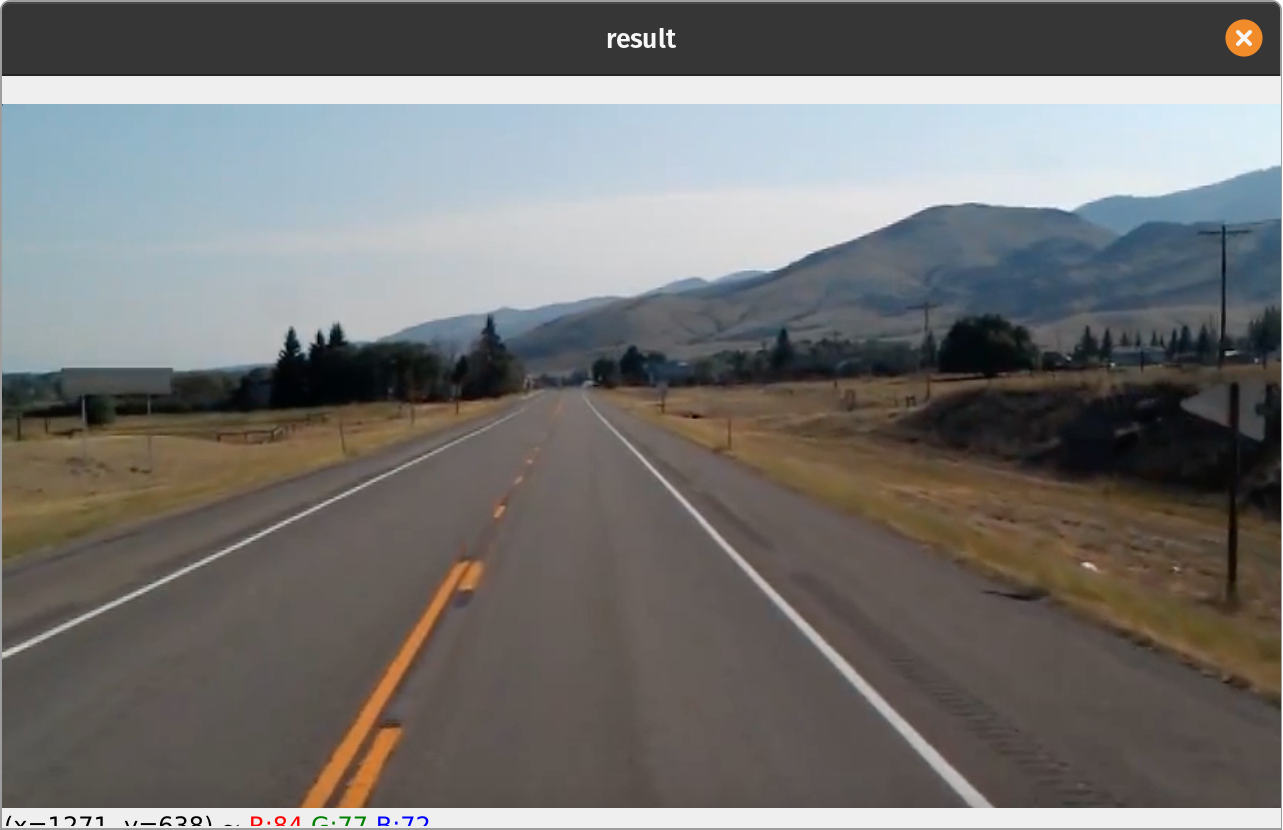
\includegraphics[width=6cm]{img/lane_detect/lane_img.png}
\caption{Original Image}
\end{minipage}
\hspace*{1cm}
\begin{minipage}{7cm}
\centering
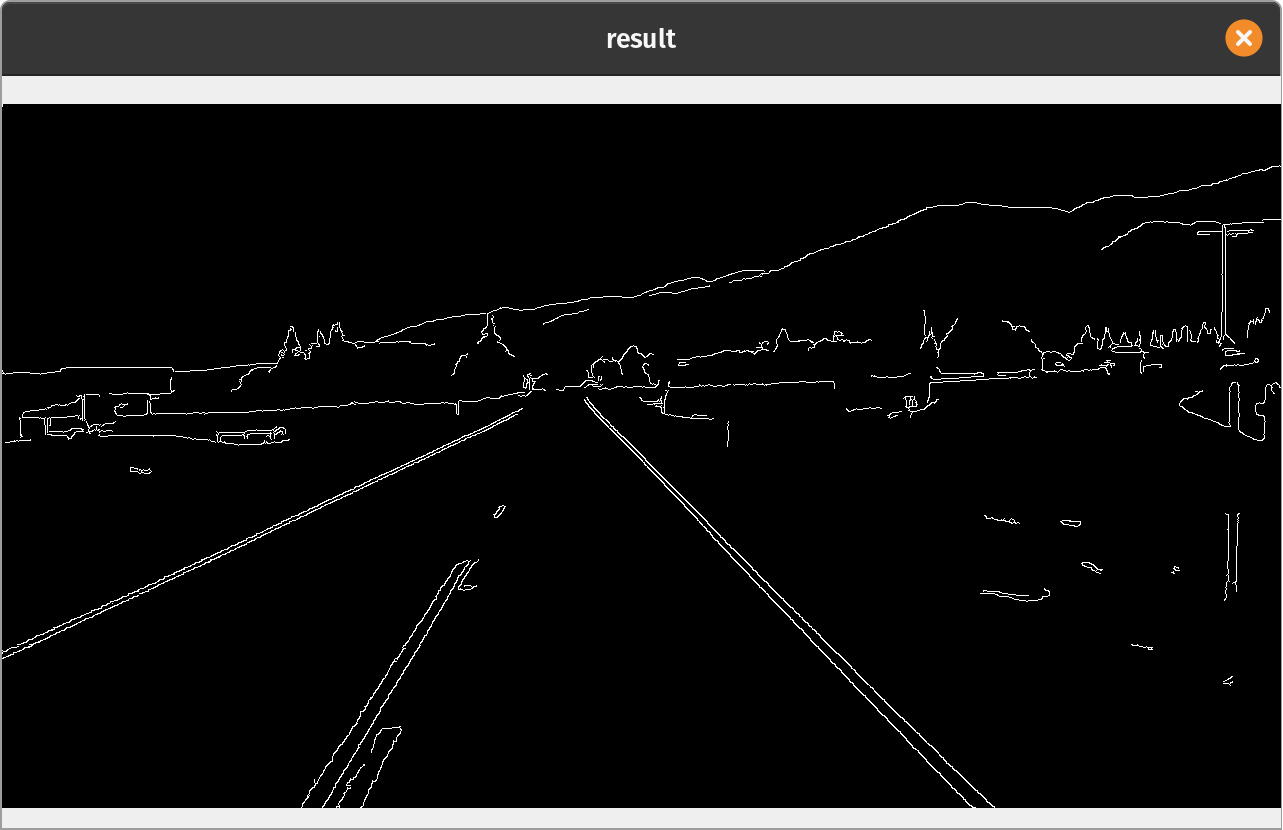
\includegraphics[width=6cm]{img/lane_detect/canny_img.png}
\caption{Gray Image after applying blur and canny-edge detection}
\end{minipage}
\end{figure}

\begin{figure}[!h]
\begin{minipage}{7cm}
\centering
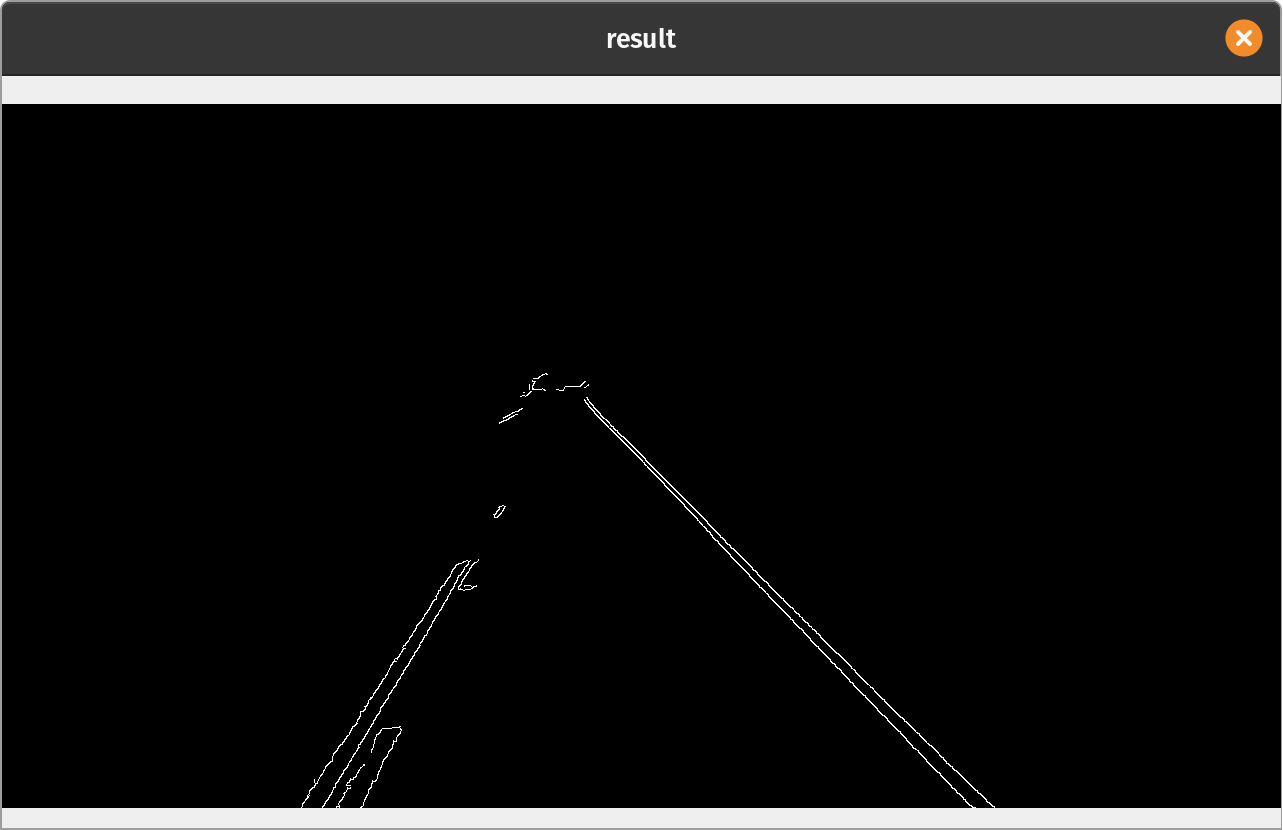
\includegraphics[width=6cm]{img/lane_detect/cropped_img.png}
\caption{We cropped the image to the center triangle}
\end{minipage}
\hspace*{1cm}
\begin{minipage}{7cm}
\centering
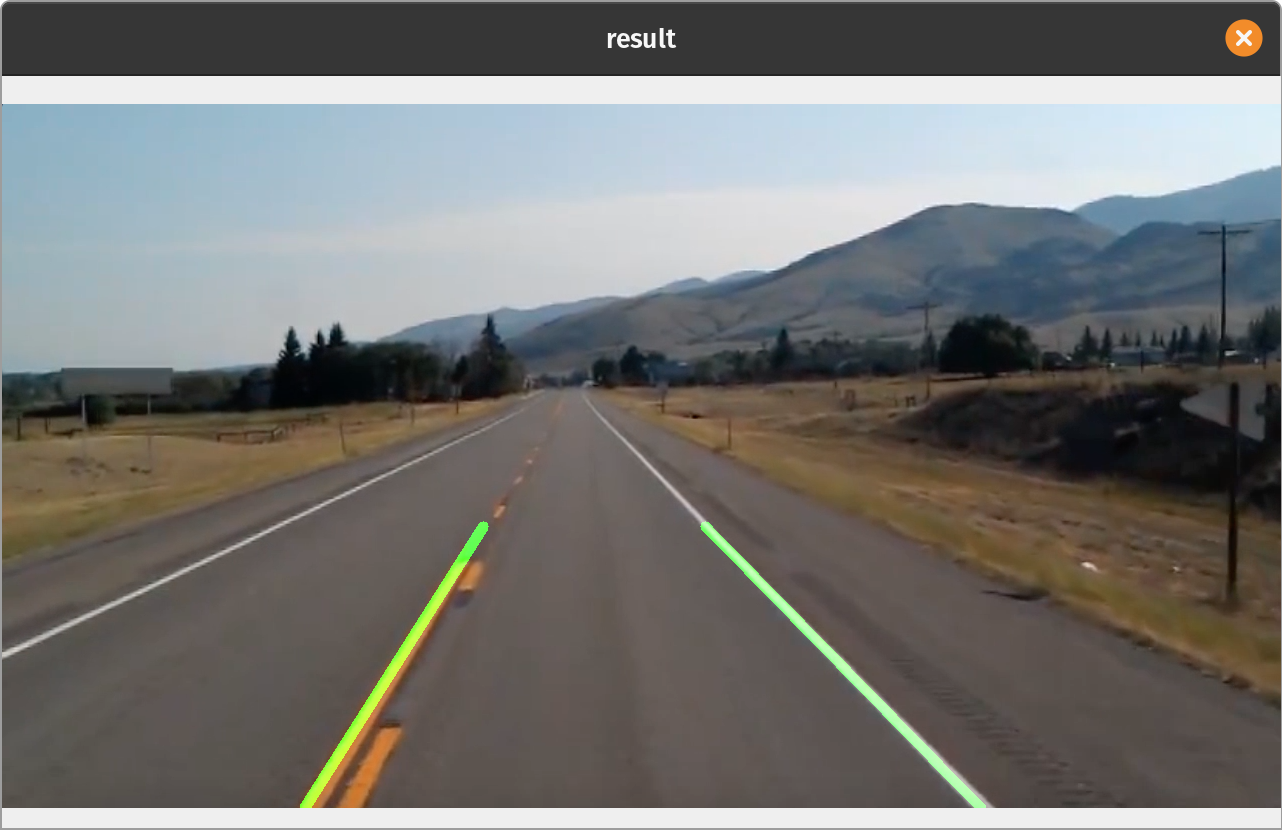
\includegraphics[width=6cm]{img/lane_detect/combo_img.png}
\caption{Final image with superposed detected lines (in green)}
\end{minipage}
\end{figure}

\clearpage
\subsection{TCP Client in Python}
\label{TCPClient}
\begin{python}
import socket
import base64
import requests
import socketio
import sys
import time
import json


# specify Host and Port
HOST = 'localhost'
PORT = 9091


def send_data(steering, throttle, brake):
    msg = str('{"msg_type": "control", "steering": "' +
              str(steering) + '","throttle": "' + str(throttle) +
              '","brake": "' + str(brake) + '"}').encode('utf-8')
    soc.sendall(msg)


def recv_full():
    """
    Test if the msg_type is telemetry, if yes, return the data
    """
    for _ in range(2):
        data = json.loads(soc.recv(8192).decode('utf-8'))
        if not data:
            break
        if data['msg_type'] == 'car_loaded':
            continue
        return json.loads(soc.recv(5000).decode('utf-8'))


def write_data():
    data = recv_full()
    with open('image.jpg', 'wb') as image:
        image.write(base64.b64decode(data['image']))
    with open("data.json", 'w') as f:
        json.dump(data, f)



with socket.socket(socket.AF_INET, socket.SOCK_STREAM) as soc:
    soc.connect((HOST, PORT))
    write_data()



sio = socketio.Client()
\end{python}

\subsection{Financial Management Report}
Next, you can find the financial management report we had to do, inside you will find an overview of the project and the differents approach we took for the budget repartition and the choice of the components of the car.
\includepdf[pages=-]{pdf/PA_finance.pdf}

\end{appendices}
%%% Résumé en 3 langues du projet

\section{Résumé en trois langues}
\section*{Français}

Durant le dispositif Activ'ESAIP, notre équipe, constituée de Valentin \textsc{Carrillo}, Romain \textsc{Girou} et Cyprien \textsc{Barbault}, a été amené à travailler avec Panorama Performance. Cette TPE est spécialisée dans l'aide à la performance industrielle. La mission qu'elle nous a confiée est la suivante : est-il possible de digitaliser un de leurs outils, le séquenceur, et d'en faire une solution viable tant pour leur client que pour Panorama. Après une semaine de recherche, nous avons décidé de développer une POC en Flutter pour montrer la faisabilité d'un tel projet. En parallèle, nous avons également rédigé un business modèle présentant les différentes options de financement et les coûts associés. En suivant les lignes de conduite de la méthode agile, nous avons pu rendre des livrables réguliers à nos tuteurs et leur délivrer en temps et en heure une version de test. Suite à cette séance d'essai, Panorama Performance nous a annoncé vouloir présenter un MVP à ses plus fidèles clients pour récolter leurs avis et lancer ou non la production.

\section*{English}

During activ'ESAIP, our team, made up of Valentin \textsc{Carrillo}, Romain \textsc{Girou} and Cyprien \textsc{Barbault}, was brought to work with Panorama Performance. This TPE specialises in industrial performance support. The mission she entrusted to us is this: is it possible to digitize one of their tools, the sequencer, and make it a viable solution for both their client and Panorama. After a week of research, we decided to develop a flutter POC to show the feasibility of such a project. At the same time, we have also drafted a business model presenting the different financing options and associated costs. By following the agile method, we were able to return regular deliverables to our tutors and deliver them a test version on time. Following this test session, Panorama Performance announced that it wanted to present an MVP to its most loyal customers to collect their opinions and launch or not the production.

\section*{Español}

Durante el dispositivo activ'ESAIP, nuestro equipo, compuesto por Valentin \textsc{Carrillo}, Romain \textsc{Girou} y Cyprien \textsc{Barbault}, trabajó con Panorama Performance. Esta TPE se especializa en la ayuda al rendimiento industrial. La misión que nos ha confiado es la siguiente: es posible digitalizar una de sus herramientas, el secuenciador, y hacer de ella una solución viable tanto para su cliente como para Panorama. Después de una semana de investigación, decidimos desarrollar una POC en Flutter para demostrar la viabilidad de tal proyecto. Paralelamente, también hemos elaborado un modelo de negocio que presenta las diferentes opciones de financiación y los costes asociados. Siguiendo las líneas del método ágil, hemos podido entregar entregas regulares a nuestros tutores y entregarles a tiempo una versión de prueba. Tras esta sesión de prueba, Panorama Performance nos ha anunciado que quiere presentar un MVP a sus clientes más fieles para recoger sus opiniones y lanzar o no la producción.

\end{document}
